%%%%%%%%%%%%%%%%%%%%%%% file template.tex %%%%%%%%%%%%%%%%%%%%%%%%%
%
% This is a general template file for the LaTeX package SVJour3
% for Springer journals.          Springer Heidelberg 2010/09/16
%
% Copy it to a new file with a new name and use it as the basis
% for your article. Delete % signs as needed.
%
% This template includes a few options for different layouts and
% content for various journals. Please consult a previous issue of
% your journal as needed.
%
%%%%%%%%%%%%%%%%%%%%%%%%%%%%%%%%%%%%%%%%%%%%%%%%%%%%%%%%%%%%%%%%%%%
%
% First comes an example EPS file -- just ignore it and
% proceed on the \documentclass line
% your LaTeX will extract the file if required
%
\RequirePackage{fix-cm}
%
%\documentclass{svjour3}                     % onecolumn (standard format)
%\documentclass[smallcondensed]{svjour3}     % onecolumn (ditto)
%\documentclass[smallextended]{svjour3}       % onecolumn (second format)
%\documentclass[twocolumn]{svjour3}          % twocolumn
%
\documentclass[runningheads, a4paper, 10pt]{llncs}

%\smartqed  % flush right qed marks, e.g. at end of proof
%
\usepackage{graphicx}
\usepackage{caption}
\usepackage{subcaption}
\usepackage{url}
\usepackage{amssymb}
\usepackage{amsmath}
\usepackage{booktabs}    
\usepackage{cite}    
\usepackage{comment}    
\usepackage{subfig}    
\usepackage{tabu}

\usepackage{multirow}

%\usepackage[T1]{fontenc}
%\usepackage{libertine}%% Only as example for the romans/sans fonts
%\usepackage[scaled=0.85]{beramono}

\usepackage{todonotes} % while work in progress
\usepackage{listings} % for source code

% Code listing settings
\definecolor{mygreen}{rgb}{0,0.6,0}
\definecolor{mygray}{rgb}{0.5,0.5,0.5}

\lstset{ %
  backgroundcolor=\color{white},
  basicstyle=\sffamily\footnotesize,
  breakatwhitespace=false,
  breaklines=true,
  captionpos=b,
  commentstyle=\color{mygreen},
  language=[x86masm]Assembler,
  keywordstyle=\color{blue},
  keywords={brcc, lsl, eor, add, mov, ldi, st, ld, NOP},
  deletekeywords={if,label},
  escapeinside={@}{@},          % if you want to add LaTeX within your code
  %extendedchars=true,              % lets you use non-ASCII characters; for 8-bits encodings only, does not work with UTF-8
  %frame=single,	                   % adds a frame around the code
  keepspaces=true,
  numbers=left,                    % where to put the line-numbers; possible values are (none, left, right)
  numbersep=5pt,                   % how far the line-numbers are from the code
  numberstyle=\tiny\color{mygray}, % the style that is used for the line-numbers
  rulecolor=\color{black},         % if not set, the frame-color may be changed on line-breaks within not-black text (e.g. comments (green here))
  showspaces=false,                % show spaces everywhere adding particular underscores; it overrides 'showstringspaces'
  showstringspaces=false,          % underline spaces within strings only
  showtabs=false,                  % show tabs within strings adding particular underscores
  stepnumber=1,                    % the step between two line-numbers. If it's 1, each line will be numbered
  stringstyle=\color{mymauve},     % string literal style
  tabsize=2,	                   % sets default tabsize to 2 spaces
  title=\lstname                   % show the filename of files included with \lstinputlisting; also try caption instead of title
}


\usepackage{float}
\hyphenation{en-co-ded}

%
% \usepackage{mathptmx}      % use Times fonts if available on your TeX system
%
% insert here the call for the packages your document requires
%\usepackage{latexsym}
% etc.
%
% please place your own definitions here and don't use \def but
% \newcommand{}{}
%
% Insert the name of "your journal" with
% \journalname{myjournal}
%
\begin{document}
\bibliographystyle{plain}


\title{Mind the Gap: Towards Secure 1st-order Masking in Software
\thanks{
Funding acknowledgement Removed for submission (anonymyty requirement)
  % The work described in this paper has been supported 
  % by the Netherlands Organization for Scientific Research NWO under project ProFIL (628.001.007).
}}

%\titlerunning{Short form of title}        % if too long for running head

\author{Author list removed for submission}

\institute{Institute list removed for submission}

\maketitle

\begin{abstract}
Software-based cryptographic implementations are vulnerable to side-channel analysis. 
Implementors often opt for masking countermeasures to protect against these types of attacks.
Masking countermeasures ensure theoretical protection against value-based leakages. However, the practical effectiveness of masking is halted by 
physical effects such as glitches and distance-based leakages, which violate the \emph{independent leakage assumption} (ILA) and result in security order reductions. This paper aims to address this gap between masking theory and practice in the following threefold manner. First, we perform an in-depth investigation of the device-specific effects that invalidate ILA in the AVR microcontroller ATMega163. Second, we provide an automated tool, capable of detecting ILA violations in AVR assembly code. Last, we craft the first (to our knowledge) \emph{``hardened''} 1st-order ISW-based, masked Sbox implementation, which is capable of resisting 1st-order, univariate side-channel attacks. Enforcing the ILA in the masked RECTANGLE Sbox requires $1319$ clock cycles, i.e. a $15$-fold increase compared  to a naive 1st-order ISW-based implementation. 

\keywords{Masking, AVR, verification tool, simulator, independent leakage assumption, distance-based leakage, RECTANGLE, SCA }

\end{abstract}

\section{Introduction}
Nowadays, the explosive growth of the ``Internet of Things'' (IoT) is reshaping modern society, pervading its infrastructure and communications.
The rapid price drop in IoT components has transformed everyday products, enhancing them with network connectivity and information exchange capabilities. Amidst this new status quo, devices, ranging from cheap sensors to expensive vehicles, are required to maintain a heightened level of theoretical and physical security.

For instance, side-channel attacks (SCA) allow adversaries to recover sensitive data, by observing and analyzing the
physical characteristics and emanations of a cryptographic implementation~\cite{DBLP:conf/crypto/KocherJJ99}. Such physical attacks motivated research towards countermeasures that perform noise amplification, thus hindering the adversary's recovery capabilities. A common choice for provably secure, noise-amplifying software countermeasure is masking~\cite{DBLP:conf/crypto/ChariJRR99,DBLP:conf/crypto/IshaiSW03}. Masking employs secret-sharing techniques that establish theoretical security against the value-based leakage model. Rephrasing, masking secures implementations against adversaries that can only extract information about the value being processed at a given time. This underlying assumption is often referred to as the \emph{independent leakage assumption} (ILA)~\cite{DBLP:conf/eurocrypt/RenauldSVKF11}. Unfortunately, the exact values under manipulation are not always visible at a given layer of abstraction, e.g. at assembly code and such a limited adversarial model is not applicable in many practical, software-based scenarios. For instance, devices often exhibit \emph{distance-based leakages}, which can reduce the security of the masking countermeasure~\cite{DBLP:conf/cardis/BalaschGGRS14, DBLP:journals/iacr/GrootPPSB16}. Likewise, coupling effects~\cite{DBLP:conf/eurocrypt/RenauldSVKF11} and glitches~\cite{DBLP:conf/ches/MangardS06} can pose similar security hazards.

This work attempts to bridge the gap between theory and practice in the masking countermeasure with the following threefold contribution. First, we investigate several effects that violate ILA in an ATMega163 microcontroller and subsequently, we establish solutions that mitigate these issues. Second, we use this knowledge in order to build an assembly-oriented tool that is capable of detecting ILA violations in AVR-based masked implementations. Third, assisted by the developed tool, we craft the first (to our knowledge) 1st-order masked implementation in ATMega163 that is capable of resisting 1st-order, univariate attacks. In other words, we enforce the ILA in order to severely limit the informativeness of 1st-order leakages, forcing the adversary to resort to 2nd-order attacks. As a proof of concept, we develop a ``hardened" 1st-order, ISW-based~\cite{DBLP:conf/crypto/IshaiSW03}, bitsliced Sbox for the RECTANGLE cipher~\cite{DBLP:journals/chinaf/ZhangBLR0V15}. The ``hardened'' implementation requires 1319 clock cycles, a 15-fold increase compared to a ``naive" 1st-order, ISW-based, bitsliced Sbox of the same cipher. 

The paper is organized as follows. In Section~\ref{sec:background}, we provide preliminaries w.r.t. masking, the experimental setup and the evaluation techniques we employ. In Section~\ref{sec:ila_effects} we offer a detailed description of all the ILA-breaching effects that we have identified in ATMega163. 
Section~\ref{sec:tool} discusses the development of the assembly verification tool. Section~\ref{sec:rectangle} details the construction of a ``hardened'' RECTANGLE, 1st-order masked Sbox for ATMega163. We conclude and discuss future work in Section~\ref{sec:conclusions}.



\section{Background} \label{sec:background}
\subsection{Boolean Masking \& Order Reduction}
Chari et al., Goubin et al. and Messerges~\cite{DBLP:conf/crypto/ChariJRR99,DBLP:conf/ches/GoubinP99,DBLP:conf/fse/Messerges00} were among the first to suggest splitting intermediate
values with a secret sharing scheme, in order to force attackers to analyze higher-order statistical moments. Analytically, a $d$th-order Boolean masking scheme splits a sensitive value $x$ into $d+1$ shares $(x_0, x_1, \dots, x_d)$, as shown below.
\begin{equation}
x = x_0 \oplus  x_1 \oplus \dots \oplus x_d
\end{equation}
The shares $(x_0, x_1, \dots, x_d)$ are also referred to as the $(d+1)$-family of shares corresponding to $x$~\cite{DBLP:conf/ches/RivainP10}. Given that the ILA holds and assuming sufficient noise, it has been shown that the number of traces required for a successful attack grows exponentially w.r.t. the order $d$~\cite{DBLP:conf/crypto/ChariJRR99,DBLP:conf/eurocrypt/ProuffR13}. Several implementation options have been suggested for the masking countermeasure, ranging from lookup-table techniques~\cite{DBLP:conf/eurocrypt/Coron14,DBLP:conf/ctrsa/WangVGX15} to $GF$-based circuits~\cite{DBLP:conf/crypto/IshaiSW03,DBLP:journals/iacr/CanrightB09,DBLP:conf/ches/RivainP10,cryptoeprint:2016:264}.

In parallel with the development of masked implementations, side-channel research focused on the practical evaluation of the countermeasure. Balasch et al.~\cite{DBLP:conf/cardis/BalaschGGRS14} put forward the concepts of value-based and distance-based leakages, as well as the notion of order reduction. We briefly restate their definitions below.

\vspace{0.15cm}
\noindent\textbf{Value/Distance-based leakage function} A leakage function $L(.)$ consists of a deterministic part $L_d(.)$ and random additive noise $N$. The leakage function is \emph{value-based} if $L_d(.)$ can only take arguments from the set of intermediate values produced by the masking scheme. The leakage is \emph{distance-based} if $L_d(.)$ can  take arguments from the set that contains all possible pairwise combinations of intermediate values. The combination can imply operations such as XOR, concatenation, etc.

\vspace{0.15cm}
\noindent\textbf{Order-reduction theorem} A $d$th-order secure masking scheme under value-based leakages is $\lfloor \frac{d}{2} \rfloor$th-order secure under distance-based leakages.
\vspace{0.15cm}

The applicablity of the order-reduction theorem has been verified experimentally by Balasch et al.~\cite{DBLP:conf/cardis/BalaschGGRS14} for orders $d=1,2$ in AVR-based and 8051-based devices. De Groot et al.~\cite{DBLP:journals/iacr/GrootPPSB16} have verified experimentally the theorem's applicability for orders $d=1,2$ in the ARM Cortex-M4.

\subsection{Experimental Setup \& Evaluation}
The implementation and SCA evaluation is performed on a smartcard equipped with an 8-bit, AVR-based ATMega163 microcontroller\footnote{\url{http://www.atmel.com/images/doc1142.pdf}}. 
The device features a 4.4~MHz clock, 1024 bytes of SRAM and 17 Kbytes of Flash memory. 
The acquisition of power traces is carried out using the Riscure PowerTracer\footnote{\url{https://www.riscure.com/security-tools/hardware/power-tracer}} and the Picoscope~5203 oscilloscope. The sampling rate is set at 31.5~MSamples/sec and the only post-processing applied is signal alignment.

The evaluation of the \emph{actual} security order of a masking scheme is, in general, an open problem. We often face the \emph{limited attack scope}, i.e. a given attack may not be able to exploit the available leakage due to e.g. an unsuitable choice of intermediate values or an incorrect power model. To address this problem, generic side-channel distinguishers and extensive profiling techniques have been developed~\cite{DBLP:journals/joc/BatinaGPRSV11,DBLP:conf/cardis/WhitnallOM11,DBLP:conf/eurocrypt/StandaertMY09}. In this work, we opt for the
leakage detection methodology~\cite{tvla} which prioritizes leakage detection over leakage exploitation, speeding up certain evaluation aspects. In detail, we employ the random vs. fixed, non-specific, 1st-order t-test. We perform a random vs. fixed acquisition and obtain two distinct tracesets $S_{fixed}$ and $S_{random}$, under the same encryption key. The input plaintext for $S_{fixed}$ is set to a fixed value, while for $S_{random}$, the input is uniformly random. The implementation receives the fixed or random plaintext in a non-deterministic and randomly-interleaved way (as recommended by Schneider et al. ~\cite{DBLP:conf/ches/SchneiderM15}). Following the data acquisition, the 1st-order t-test will assess whether the two sets $S_{fixed},S_{random}$ stem from the same population, using the following statistical test.
\begin{equation}
\begin{split}
H_{null}: \;\; \mu_{fixed} = \mu_{random} \\
H_{alt}: \;\; \mu_{fixed} \neq \mu_{random}
\end{split}
\end{equation}
\begin{equation}
w = \frac {\mu_{fixed} - \mu_{random}} {\sqrt{ \frac{\sigma_{fixed}^2}{n} + \frac{\sigma_{random}^2}   {m}  }  } \qquad \upsilon = \frac { (\frac{\sigma_{fixed}^2} {n}   + \frac{\sigma_{random}^2} {m}) ^2  } {\frac{\sigma_{fixed}^4} {n^2(n-1)} + \frac{\sigma_{random}^4} {m^2(m-1)}  }
\end{equation}


Parameters $\mu_{x}$ and $\sigma_{x}^2$ are the estimated mean and variance of set $x$; 
$n$ and $m$ denote sizes of sets $S_{fixed}$ and $S_{random}$ respectively. The null hypothesis $H_{null}$ is rejected at a given level of significance $\alpha$ (often set to $0.99999$), if $\lvert w \lvert >  t_{\alpha/2,\upsilon}  $, where $t_{\alpha/2,\upsilon}$ is the value of the Student t distribution with $\upsilon$ degrees of freedom. In the evaluation context, rejecting $H_{null}$ implies leakage detection, i.e. potential evidence of an ineffective masking scheme.

In this paper, we will use the t-test as a detection tool w.r.t. ILA-breaching effects and their solutions (see Section 3). Still, we will also employ 1st-order CPA methods~\cite{DBLP:conf/ches/BrierCO04} in order to demonstrate the exploitability of such effects. In order to reduce the computational cost of the evaluation, we use the memoryless formulas suggested by Schneider et al.~\cite{DBLP:conf/ches/SchneiderM15} and the incremental approach for CPA by Botinelli et al.~\cite{DBLP:journals/iacr/BottinelliB15}.



\section{ILA-Breaching Effects}\label{sec:ila_effects}

In this section, we present three effects identified in the ATMega163 microcontroller that breach ILA and pose a hazard to any masking scheme's security. Analytically, the effects below demonstrate that independent computations \emph{do not} necessarily lead to independent leakages and thus, the order-reduction theorem can become applicable.

Every effect (Sections~\ref{overwrite},~\ref{mem_remnant} and~\ref{combined_leakage}) is described as a standalone, assembly-based scenario that manipulates two 4-bit shares $x_0$, $x_1$ originating from the sensitive, key-dependent, 4-bit value $x$, such that $x=x_0 \oplus x_1$. The shares $x_0$, $x_1$ are always manipulated in a theoretically sound manner, adhering to the masking scheme's requirements, i.e. we never combine the shares directly (e.g. via an exclusive-or instruction \texttt{eor x0, x1}). 

For all the described scenarios, that are theoretically sound, we show experimentally that ILA is not fulfilled by employing 1st-order, univariate techniques. Namely, we perform correlation-based analysis~\cite{DBLP:conf/ches/BrierCO04}, computing $\rho$ between the Hamming weight of the sensitive, key-dependent value $x$ and the experimentally acquired traceset. To maintain a wide attack scope, we also use the leakage detection methodology~\cite{tvla,DBLP:conf/ches/SchneiderM15} and compute the 1st-order, random vs. fixed t-test. 
 We conclude every scenario by suggesting possible solutions that enforce ILA and verify all the proposed solutions experimentally, using a large number of traces. Restating Balasch et al.~\cite{DBLP:conf/cardis/BalaschGGRS14}, as we are always limited by the traces at hand, we cannot rule out the existence of 1st-order leakages, yet we establish that their informativeness is limited compared to 2nd-order leakages in the target device. Note that extra care is taken in order to assess all effects independently, i.e. we use the suggested solutions so as to isolate the effect under discussion from the rest.

The analyzed effects can manifest in several data storage units (e.g. registers, SRAM/Flash memory cells, I/O buffers, etc.) and may relate to different instructions of the AVR ISA\footnote{\url{http://www.atmel.com/images/Atmel-0856-AVR-Instruction-Set-Manual.pdf}}, leading to a very large number of potential scenarios. In order to maintain a feasible scope, we limit our discussion to storage units and instructions that are often encountered in the context of cryptographic implementations, i.e. SRAM memory accesses and logical instructions.
\begin{subsection}{Overwrite Effect}\label{overwrite}

The overwrite effect is observable when a share gets overwritten by a different share from the same family. For instance, if share $x_0$ in a data storage unit (register, memory cell, etc.) gets overwritten by share $x_1$, then the power consumption correlates with the number of bits switched i.e. $x_0 \oplus x_1$. This effect was observed by Daemen et al.~\cite{noteonsca} and later revisited by Coron et al.~\cite{DBLP:conf/cosade/CoronGPRRV12}.

Below, we address the most common situations in which overwriting arises during a cryptographic implementation. We perform two experiments: a register-based overwrite via the instruction \texttt{mov x0, x1}, and a memory-based overwrite via the instruction \texttt{st SRAM\_x0,  x1}. The experiments are described in Listings \ref{lst:register_overwrite},\ref{lst:memory_overwrite} and their analysis follows in Figures \ref{fig:reg_over_cpa},\ref{fig:reg_over_t},\ref{fig:mem_over_cpa},\ref{fig:mem_over_t}.

We confirm that overwriting is indeed an ILA-breaching effect, manifesting both in registers and SRAM memory. Note that the exploitability of the effect varies according to the data storage unit: in ATMega163, register-based overwriting can be exploited with roughly 500 traces (\ref{fig:reg_over_cpa}), while memory-based requires at least 40k traces (\ref{fig:mem_over_cpa}). Preventing register/memory-based overwrites is straightforward: the corresponding register/cell needs to be cleared in advance. We confirm experimentally that this solution remains secure against a $<>$k random vs. $<>$k fixed, 1st-order t-test (see Appendix).

%\begin{figure}[H]
%    \centering
%\begin{subfigure}[b]{0.40\textwidth}
%\scriptsize{\texttt{;share x0 in r17 \\
%;share x1 in r23 \\
%\textbf{mov r17,r23}}}
% \caption{\scriptsize{Register overwrite.}}
%\label{fig:reg_over_exp}
%    \end{subfigure} 
% \begin{subfigure}[b]{0.40\textwidth}
%       \scriptsize{  \texttt{;share x0 in SRAM 0x0080 \\
%;share x1 in r17  \\
%ldi r27,0x00 \\
%ldi r26,0x80 \\
%st X,r17
%}}
%     \caption{\scriptsize{Memory overwrite.}}
%\label{fig:mem_over_exp}
%    \end{subfigure}
%\caption{{Overwrite experiments}}
%\end{figure} \clearpage  
\noindent\begin{minipage}{.4\textwidth}
\lstset{caption={Register overwrite experiment.},label=lst:register_overwrite}
\begin{lstlisting}
;share x0 in r17
;share x1 in r23
mov r17,r23
;
;
\end{lstlisting}
\end{minipage}\hfill
\begin{minipage}{.4\textwidth}
\lstset{caption={Memory overwrite experiment.},label=lst:memory_overwrite}
\begin{lstlisting}
;share x0 in SRAM 0x0080
;share x1 in r17 
ldi r27,0x00
ldi r26,0x80 
st X,r17 
\end{lstlisting}
\end{minipage}



\begin{figure}[h] 
\centering
 \begin{subfigure}[b]{0.40\textwidth}
        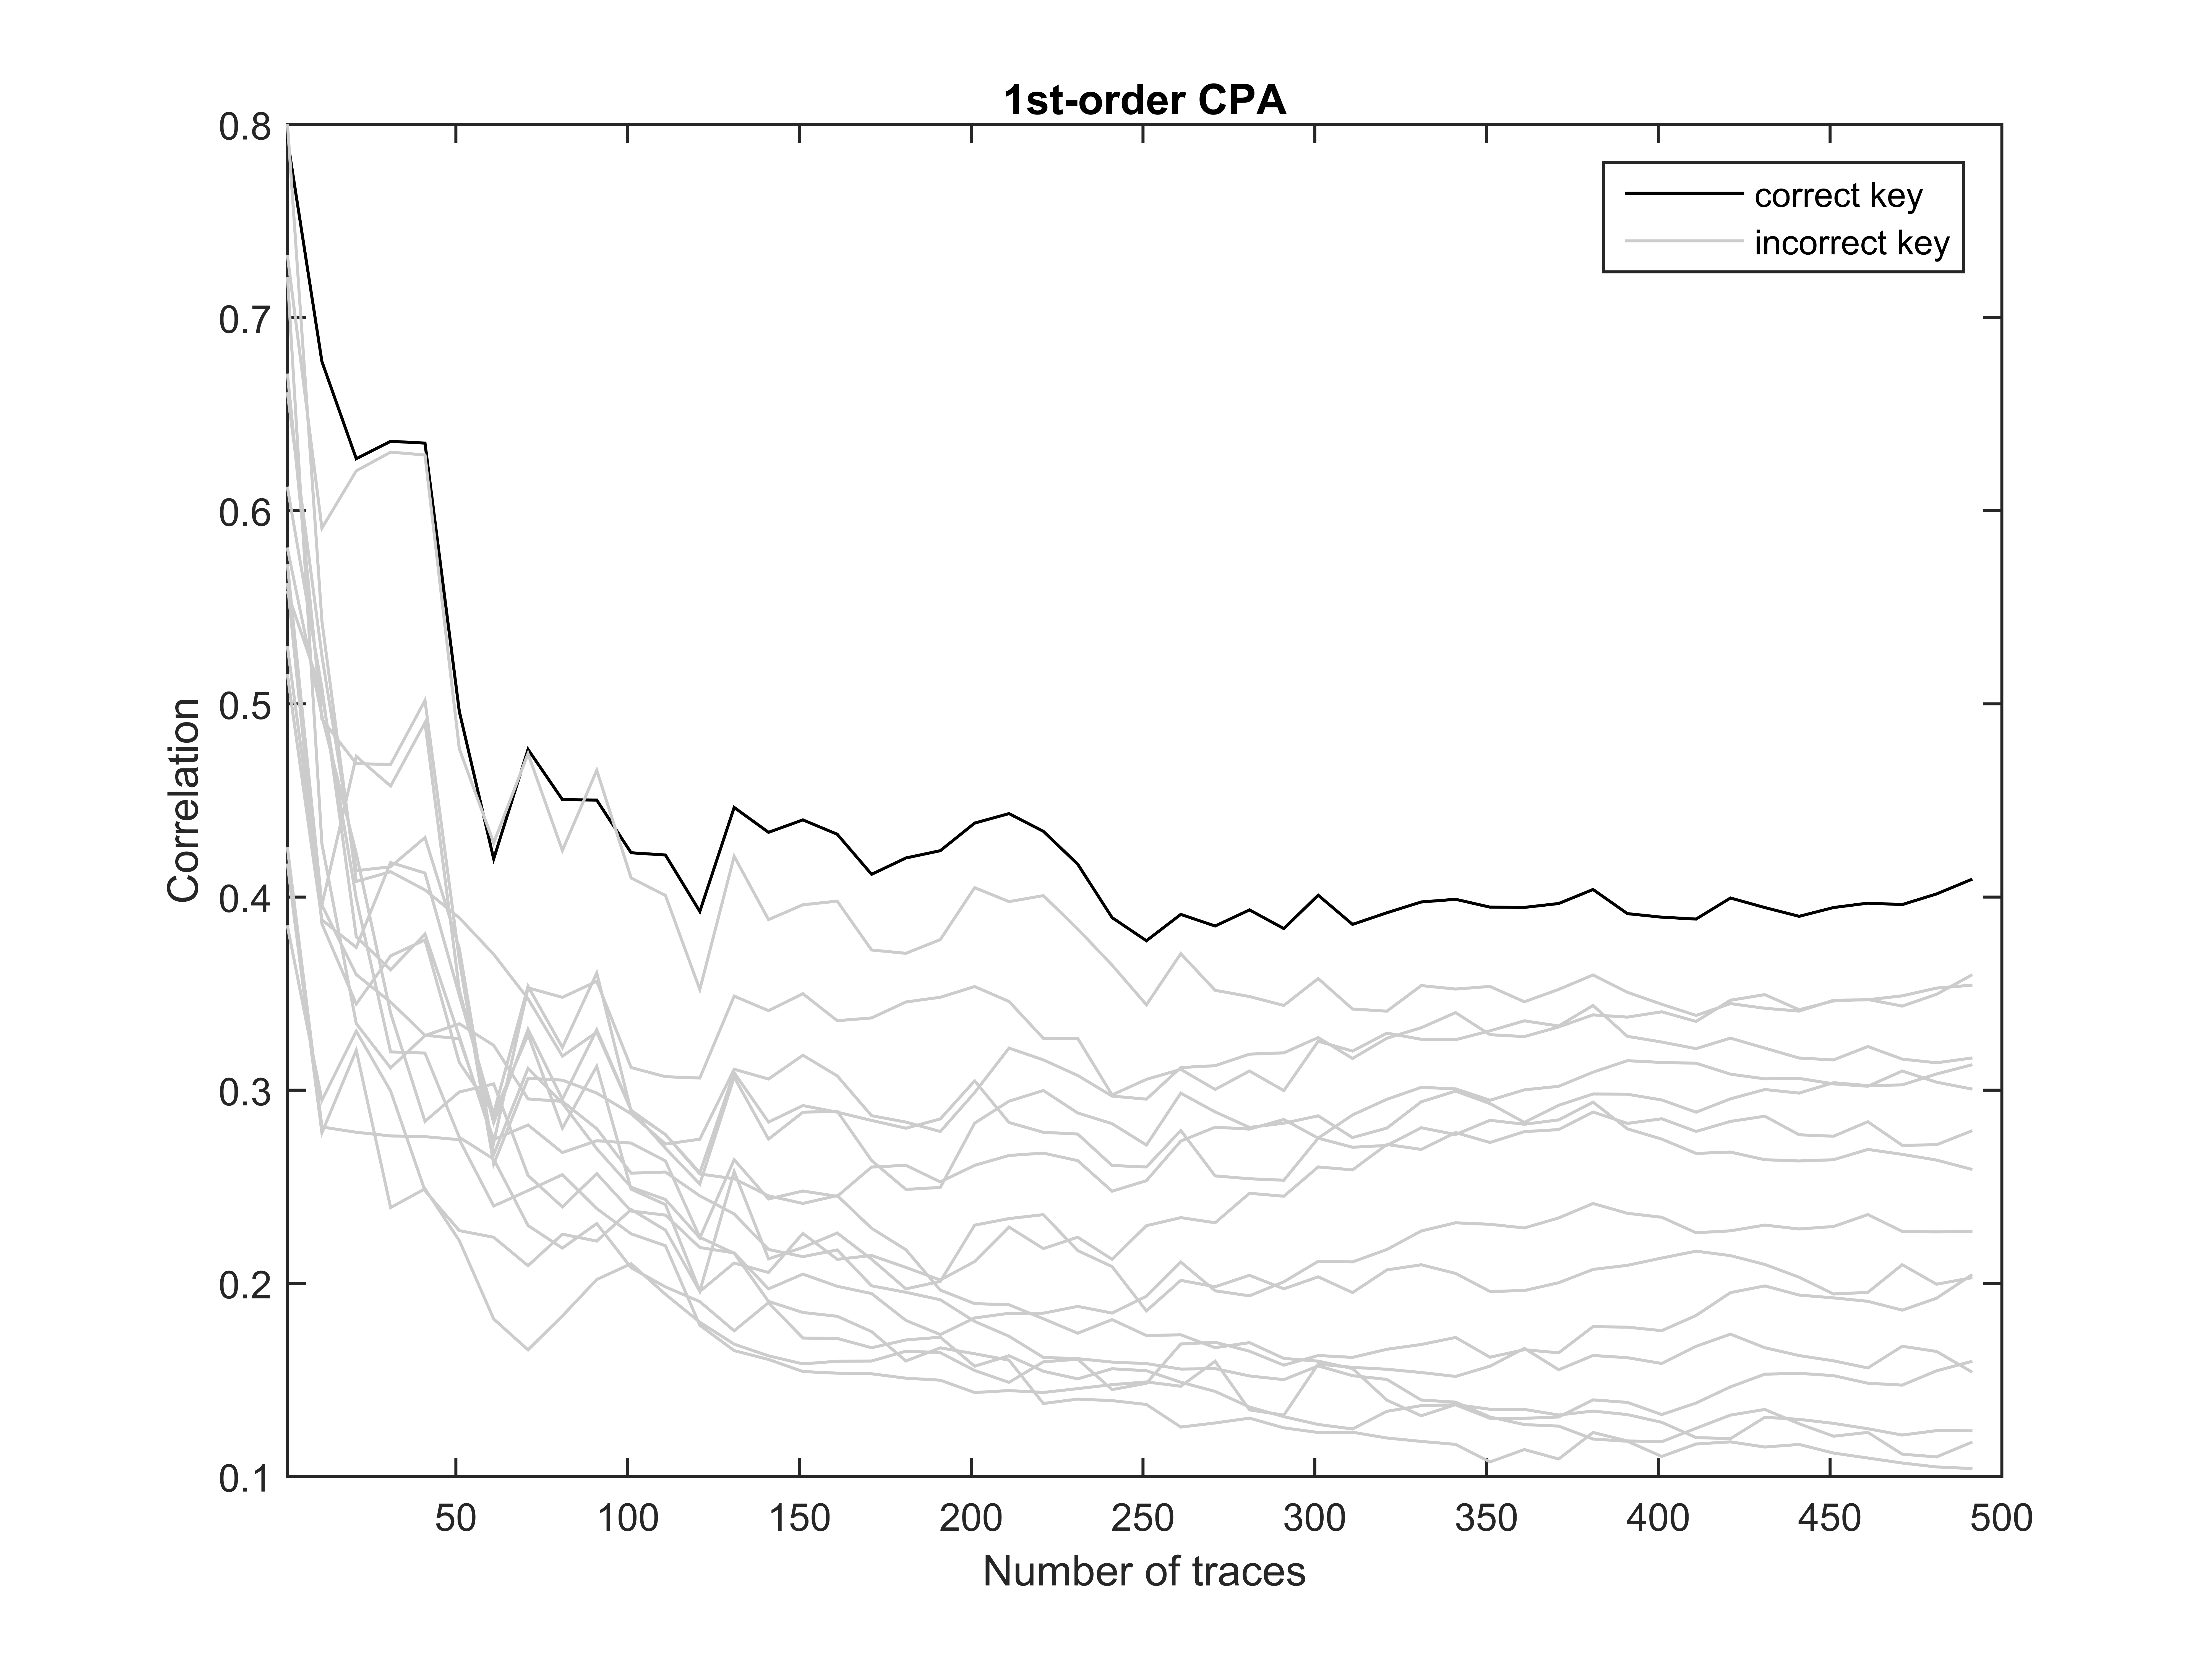
\includegraphics[width=\textwidth]{{fig/reg_over_cpa.png}}

        \caption{\scriptsize{Register overwrite, 1st-order CPA, HW model, 500 traces.}}
\label{fig:reg_over_cpa}
    \end{subfigure} \hspace{15px}
 \begin{subfigure}[b]{0.40\textwidth} 
       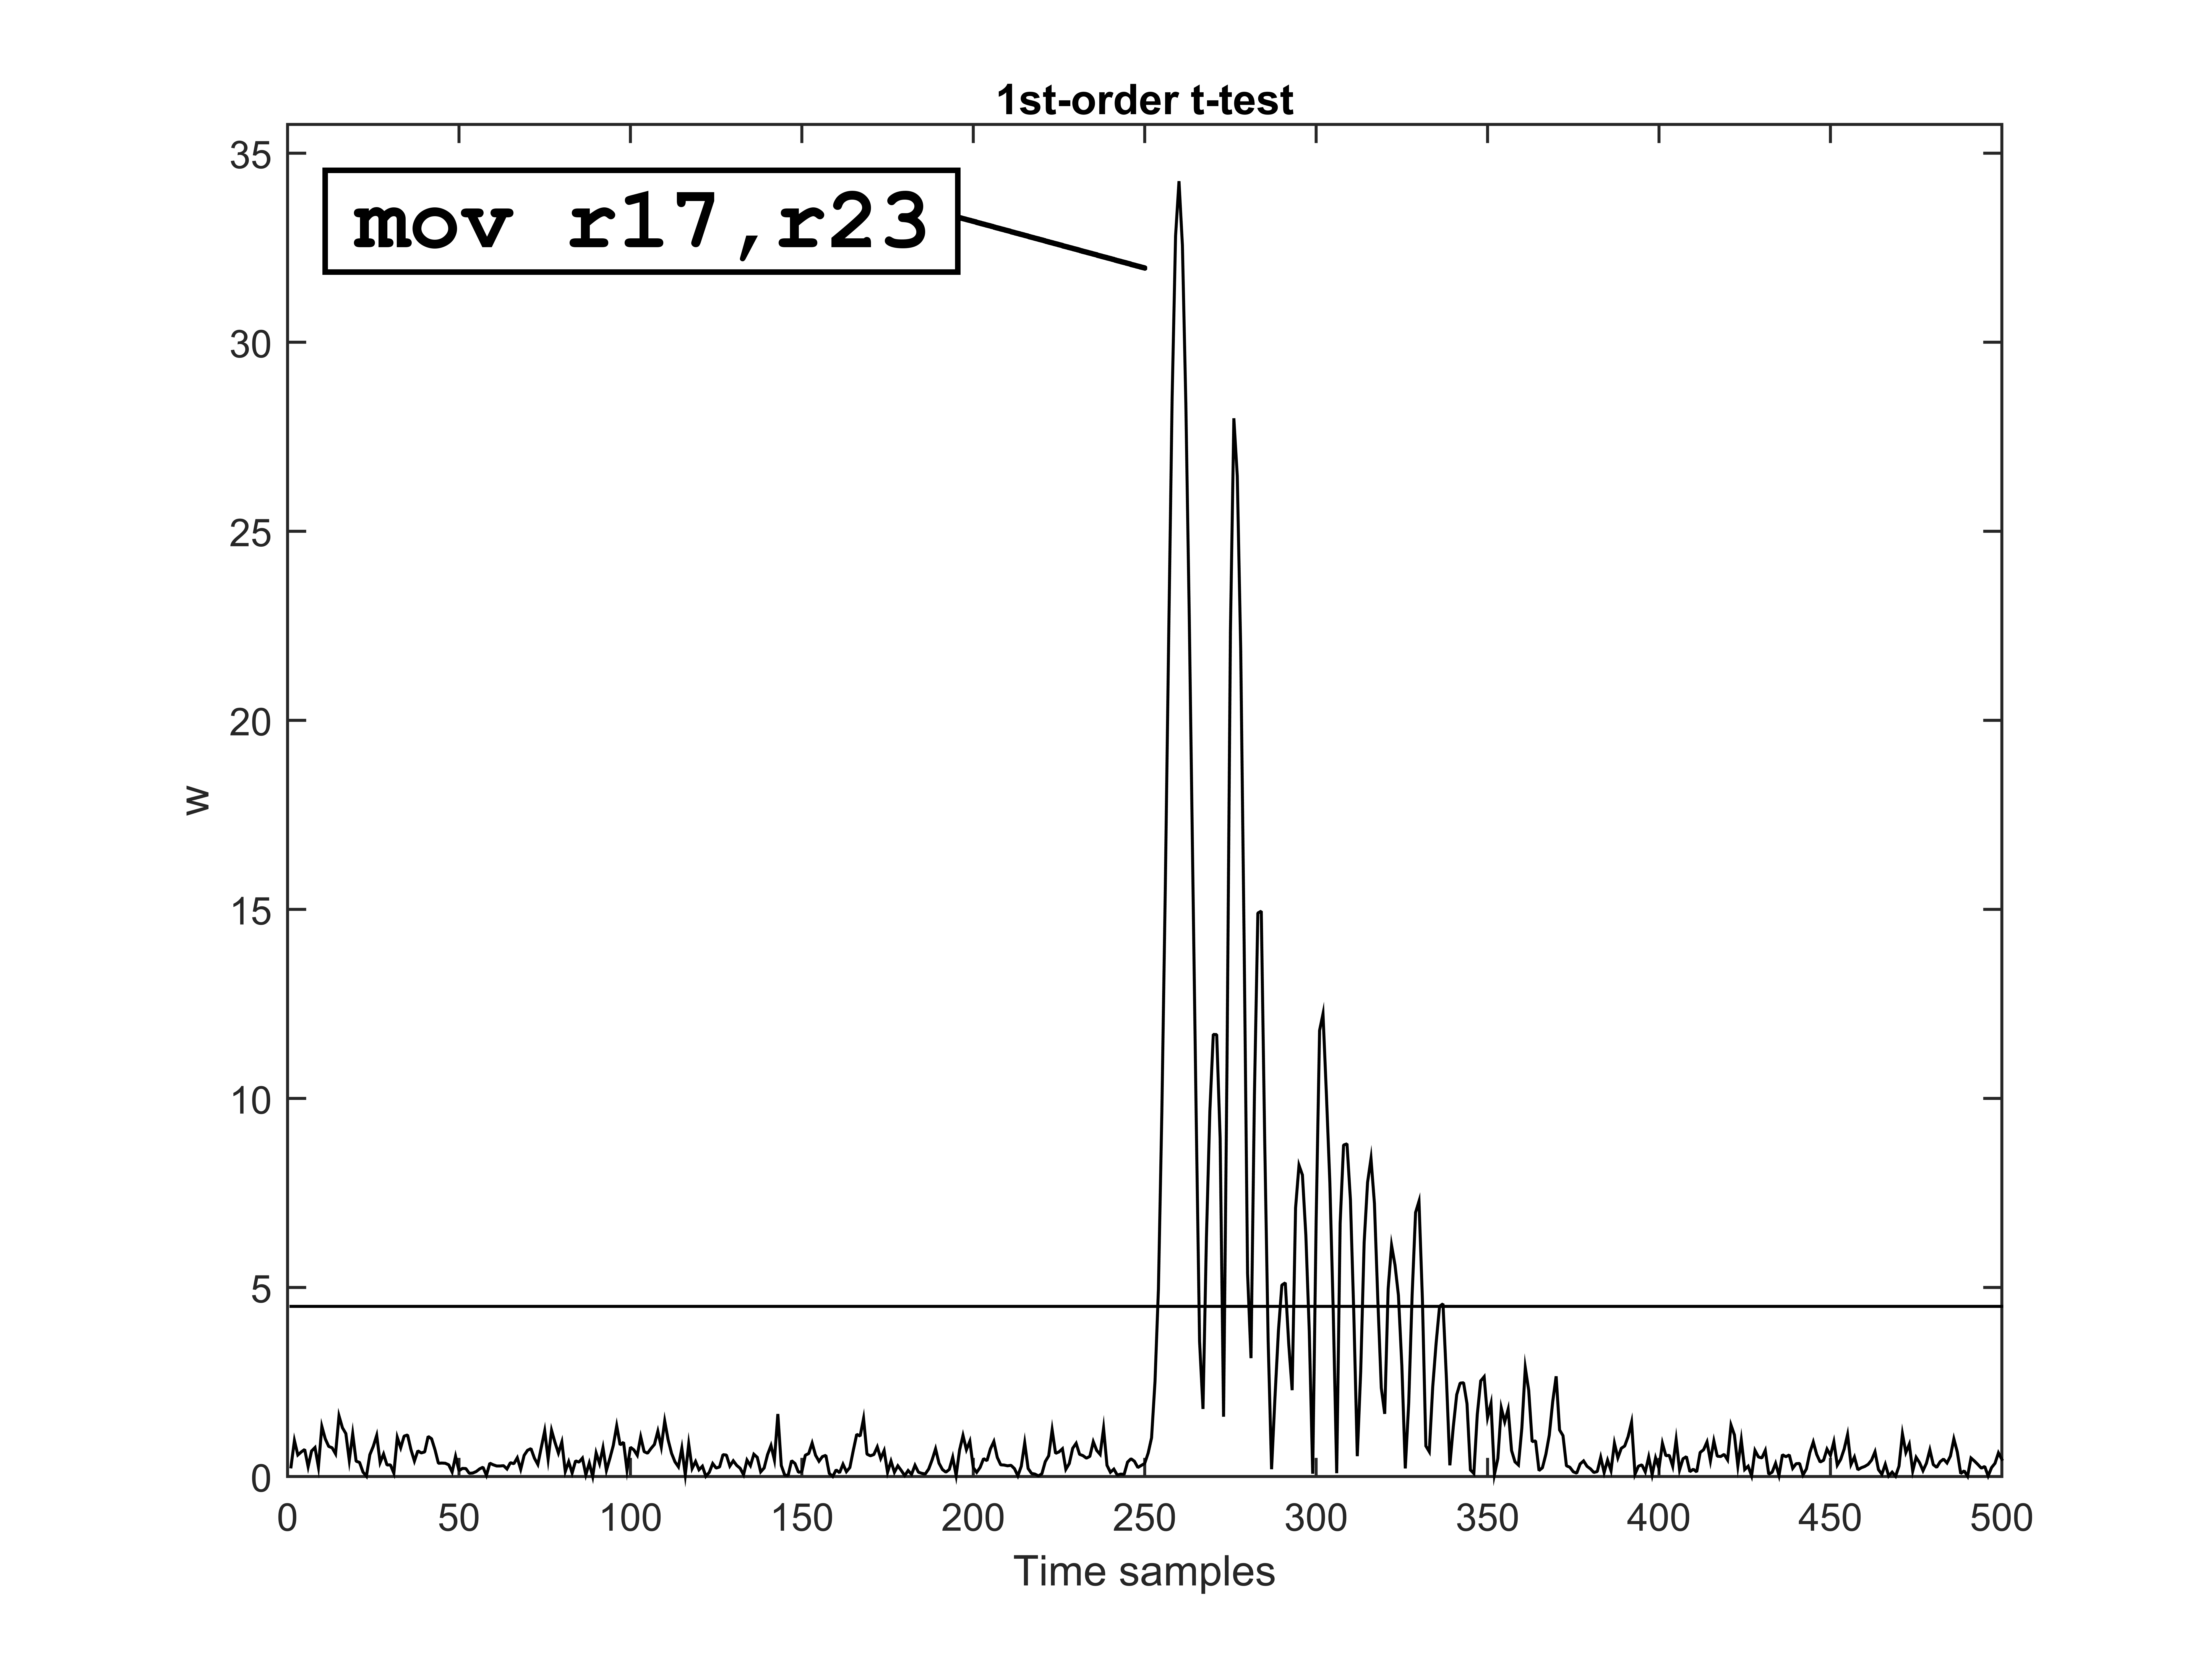
\includegraphics[width=\textwidth]{{fig/reg_over_t_an.png}}
        \caption{\scriptsize{Register overwrite, 1st-order t-test, 5k random vs. 5k fixed.}}
\label{fig:reg_over_t}
    \end{subfigure}

     %add desired spacing between images, e. g. ~, \quad, \qquad, \hfill etc. 
      %(or a blank line to force the subfigure onto a new line)
    \begin{subfigure}[b]{0.40\textwidth}
        \includegraphics[width=\textwidth]{{fig/memory_over_cpa.png}}
        \caption{\scriptsize{Memory overwrite, 1st-order CPA, HW model, 65k traces.}}
        \label{fig:mem_over_cpa}
    \end{subfigure} \hspace{15px}
    \begin{subfigure}[b]{0.40\textwidth}
        \includegraphics[width=\textwidth]{{fig/memory_over_t_an.png}}
        \caption{\scriptsize{Memory overwrite, 1st order t-test, 50k random vs. 50k fixed.}}
 \label{fig:mem_over_t}
    \end{subfigure}
    \caption{Register/memory-based overwrite effects}\label{fig:mem}
\end{figure}
\label{overwrite_section}
\end{subsection}
\begin{subsection}{Memory Remnant Effect} \label{mem_remnant}
The memory remnant effect is a leakage originating from consecutive SRAM accesses to shares of the same family. Assume that shares $x_0$, $x_1$ are stored in SRAM cells and get accessed sequentially. Naturally, the first access leaks share $x_0$ (value-based leakage), yet it also creates a ``remnant" of $x_0$. The second access will leak a combination of the share $x_1$ and the remnant $x_0$, reducing the security order. \\
%\begin{figure}[H]
 %   \centering
%\begin{subfigure}[b]{0.4\textwidth}
%\scriptsize{
  %    \texttt{;share x0 in 0x0080 \\
%;share x1 in 0x0090 \\
%ldi r27, 0x00\\
%ldi r26, 0x80\\
%ld r17, X\\
%ldi r27, 0x00\\
%ldi r26, 0x90\\
%ld r20, X
	%		}}
    %    \caption{\scriptsize{Memory remnant experiment.}}
%\label{fig:mem_rem_exp}
%    \end{subfigure} 
%\begin{subfigure}[b]{0.4\textwidth}
   %     \scriptsize{  \texttt{;share x0 in 0x0080 \\
%;share x1 in 0x0090 \\
%ldi r27, 0x00\\
%ldi r26, 0x80\\
%ld r17, X\\
%ldi r17, 0x00\\ 
%ldi r26, 0x85\\
%ld r17, X\\
%ldi r26, 0x90\\
%ld r20, X
%			}}
 %      \caption{\scriptsize{Clearing remnant experiment.}}
%\label{fig:clear_rem_exp}
%    \end{subfigure}
%\caption{{Remnant experiments}}
%\end{figure}
\begin{minipage}{.4\textwidth}
\lstset{caption={Memory remnant experiment.}, label=lst:remnant}
\begin{lstlisting}
;share x0 in 0x0080
;share x1 in 0x0090
ldi r27, 0x00
ldi r26, 0x80
ld r17, X
ldi r27, 0x00
ldi r26, 0x90
ld r20, X
;
;
\end{lstlisting}
\end{minipage}\hfill
\begin{minipage}{.4\textwidth}
\lstset{caption={Clearing remnant experiment.},label=lst:clearing_remnant}
\begin{lstlisting}
;share x0 in 0x0080
;share x1 in 0x0090
ldi r27, 0x00
ldi r26, 0x80
ld r17, X
ldi r17, 0x00 
ldi r26, 0x85
ld r17, X
ldi r26, 0x90
ld r20, X
\end{lstlisting}
\end{minipage}


\begin{figure}[H] 

 \begin{subfigure}[b]{0.40\textwidth} 
        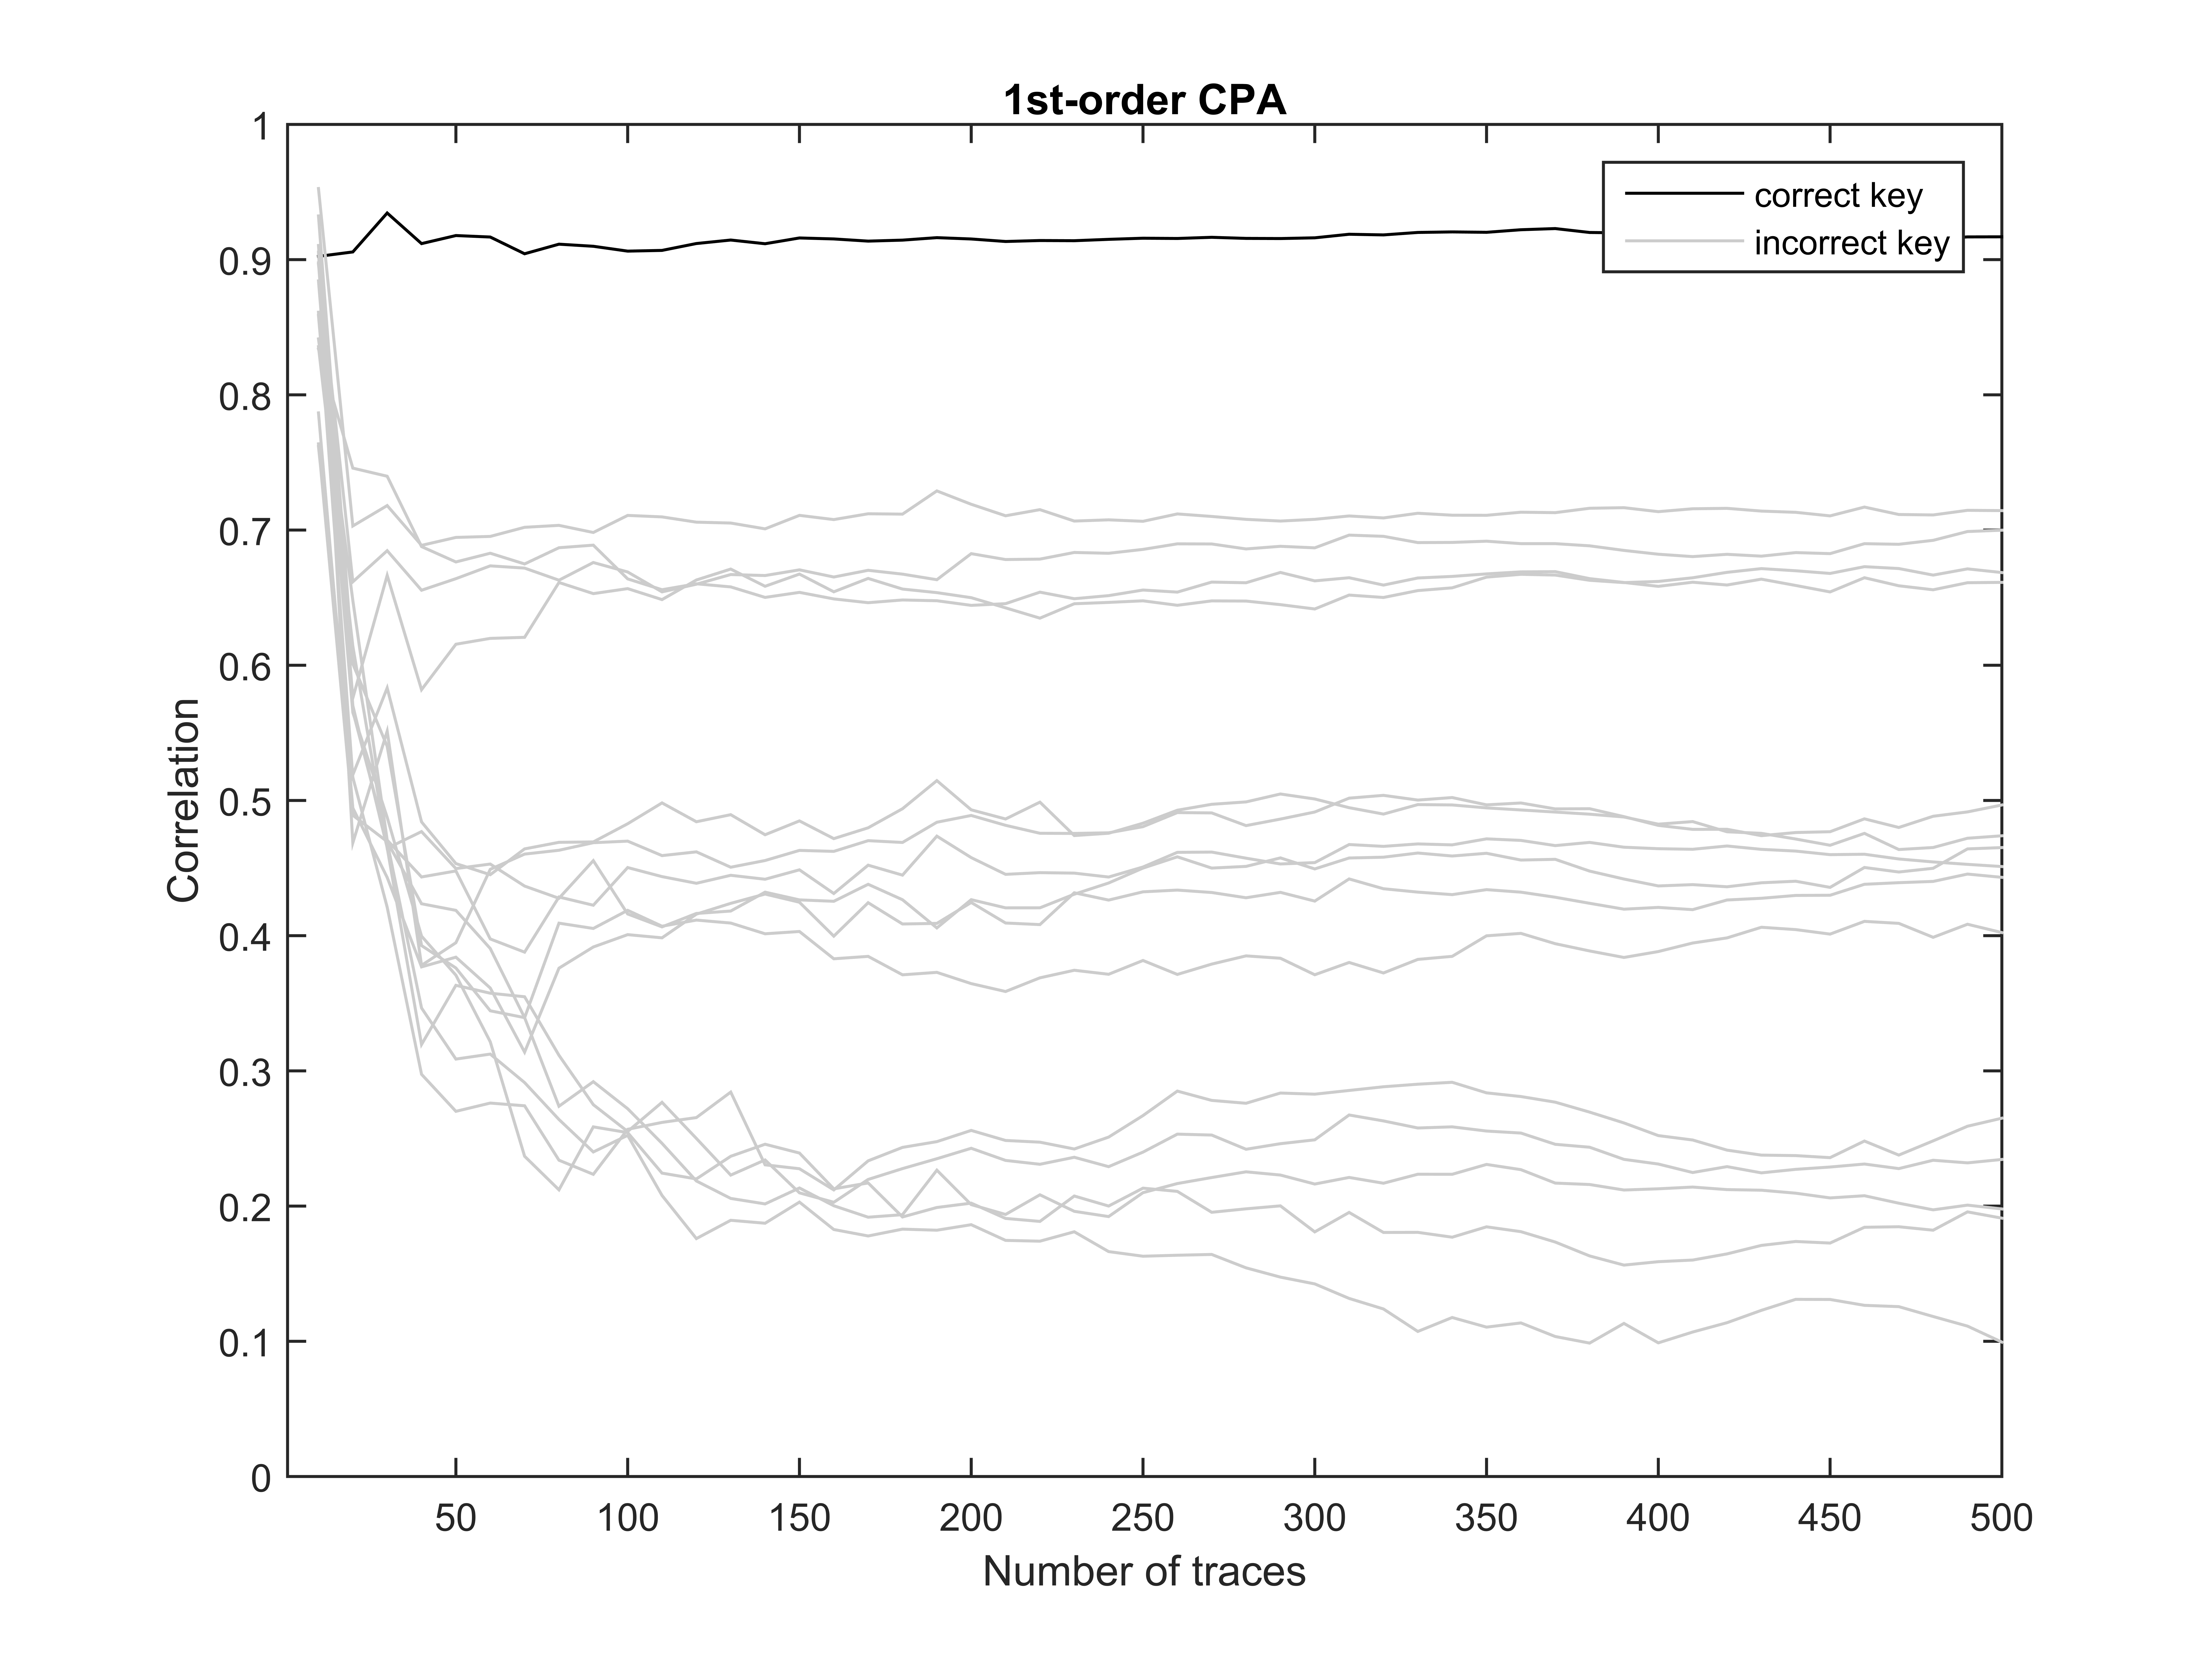
\includegraphics[width=\textwidth]{{fig/mem_rem_cpa.png}}

        \caption{\scriptsize{Memory remnant effect,1st-order CPA, HW model, 500 traces.}}
\label{fig:mem_rem_cpa}
    \end{subfigure}    \hspace{15px}
 \begin{subfigure}[b]{0.40\textwidth}
      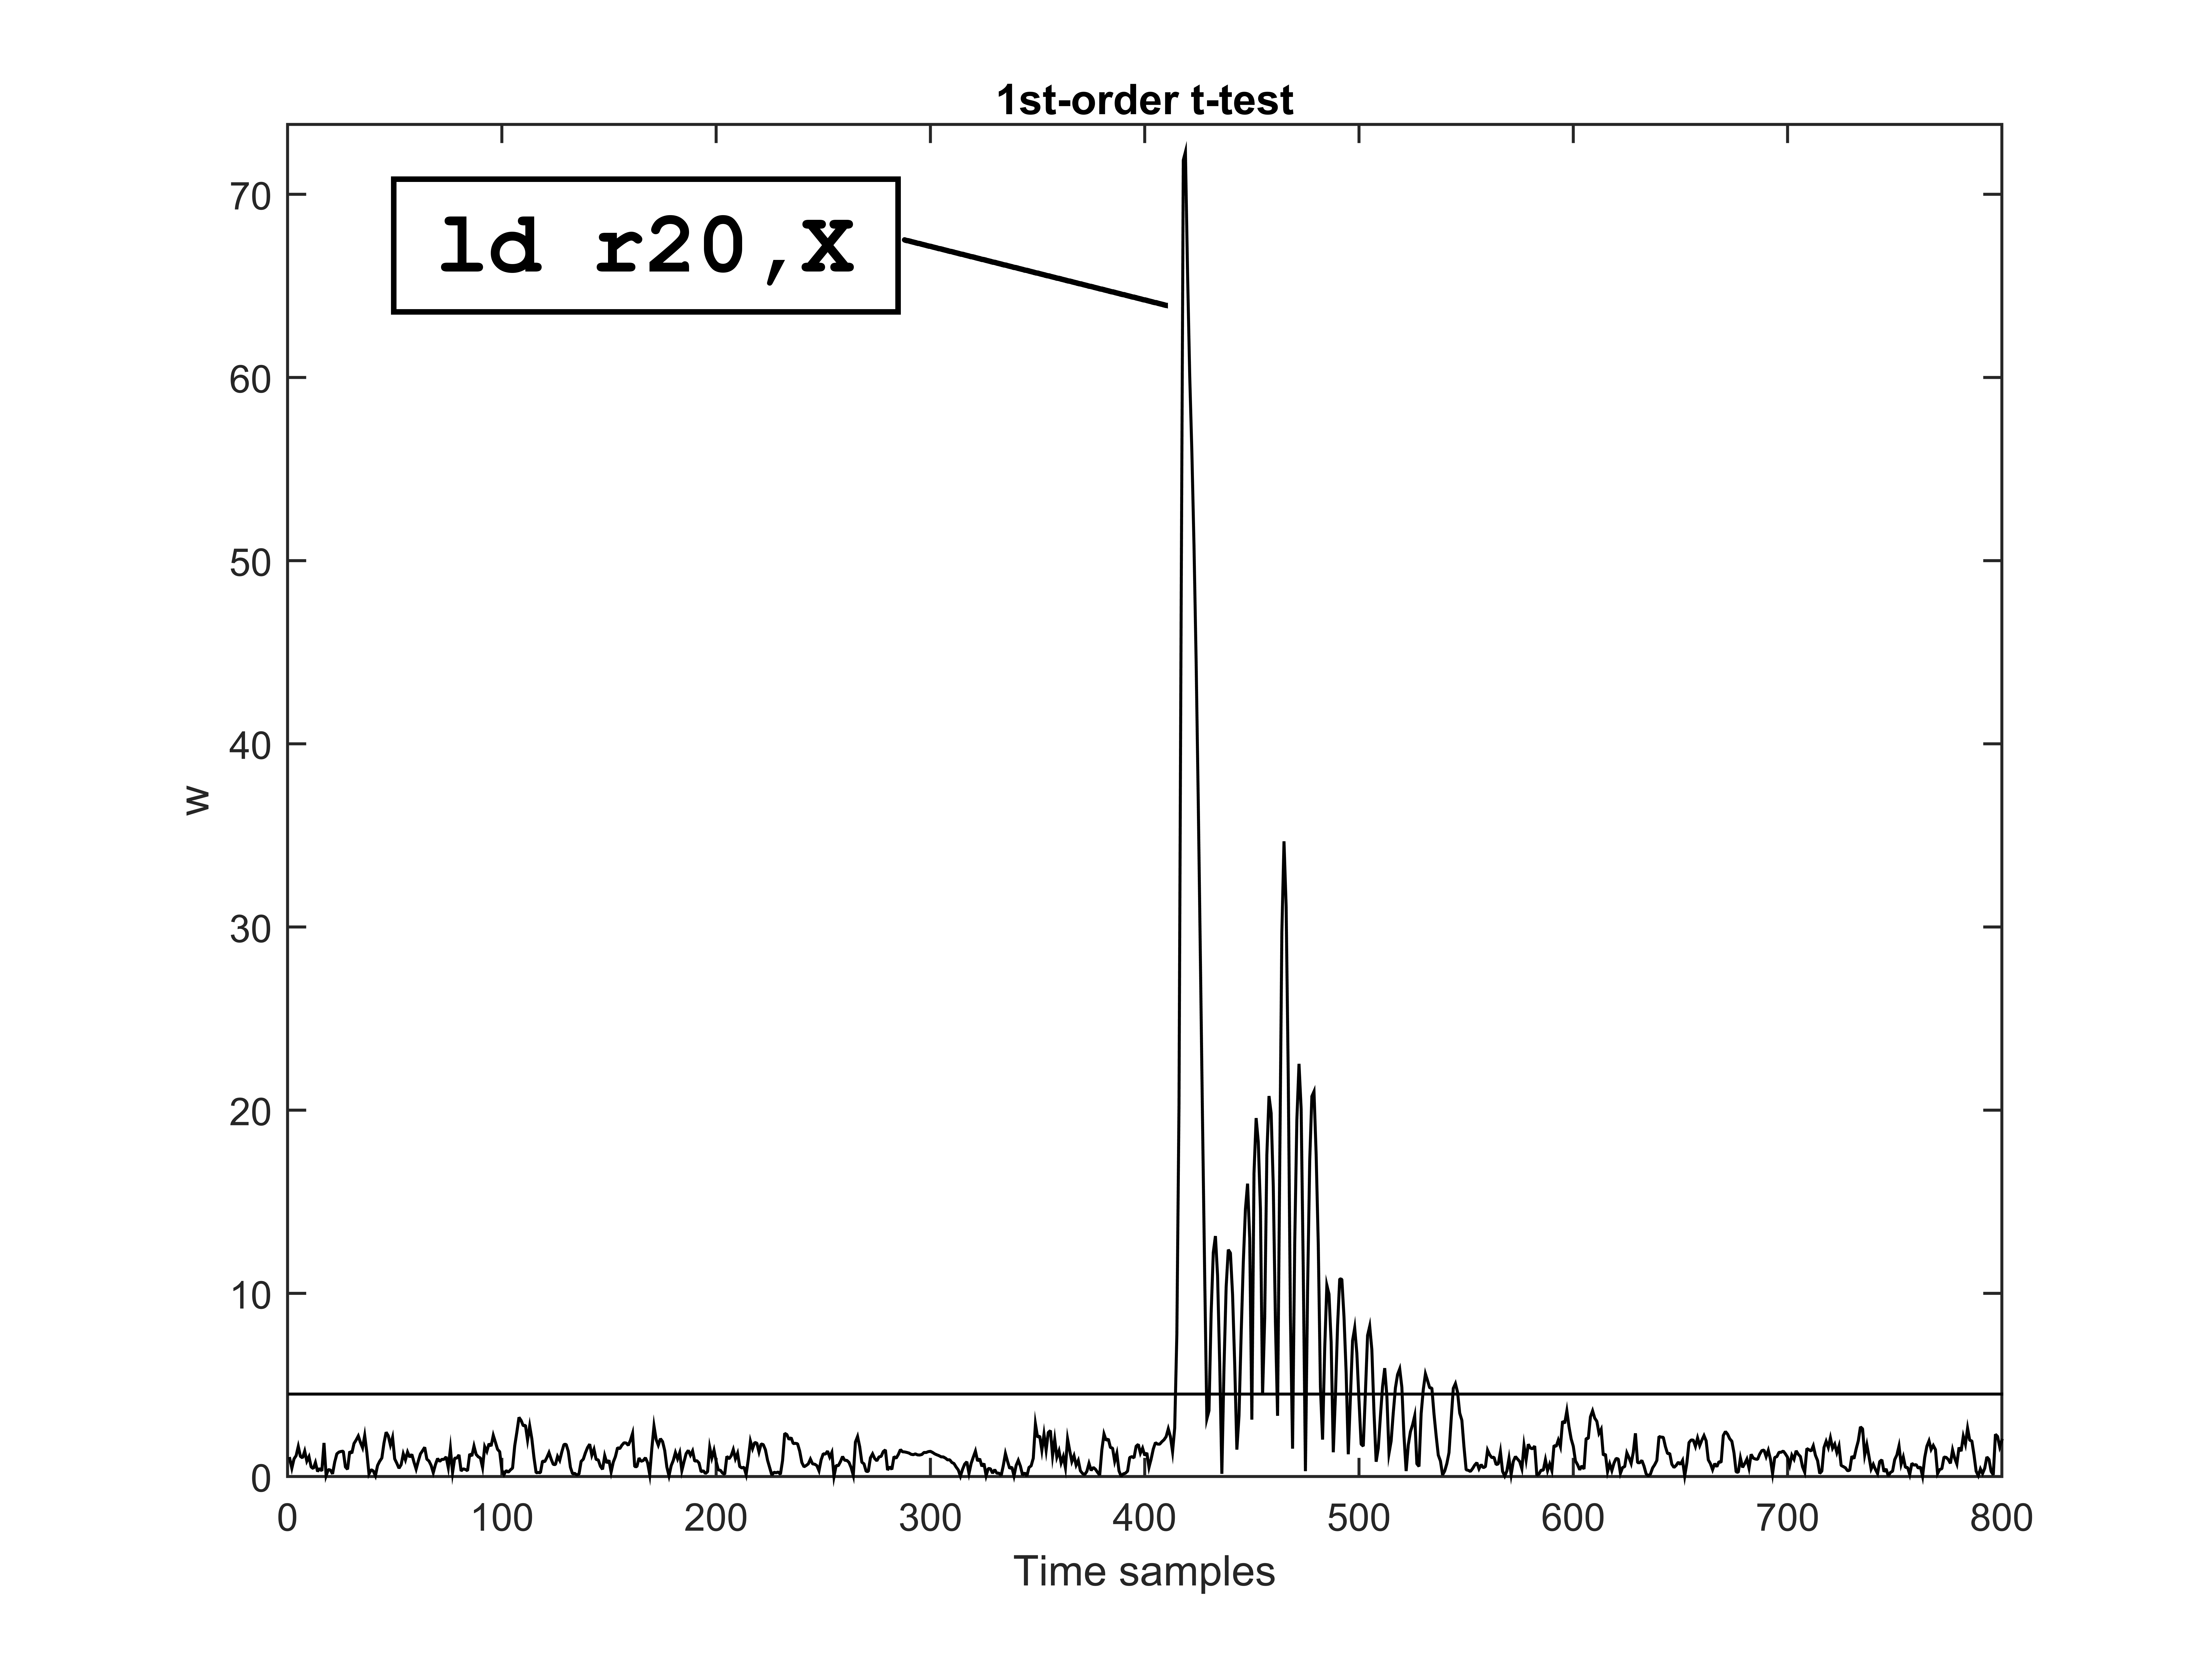
\includegraphics[width=\textwidth]{{fig/mem_rem_t_an.png}}

        \caption{\scriptsize{Memory remnant effect, 1st-order t-test, 5k random vs. 5k fixed.}}
\label{fig:mem_rem_t}
    \end{subfigure}

 \begin{subfigure}[b]{0.40\textwidth}
        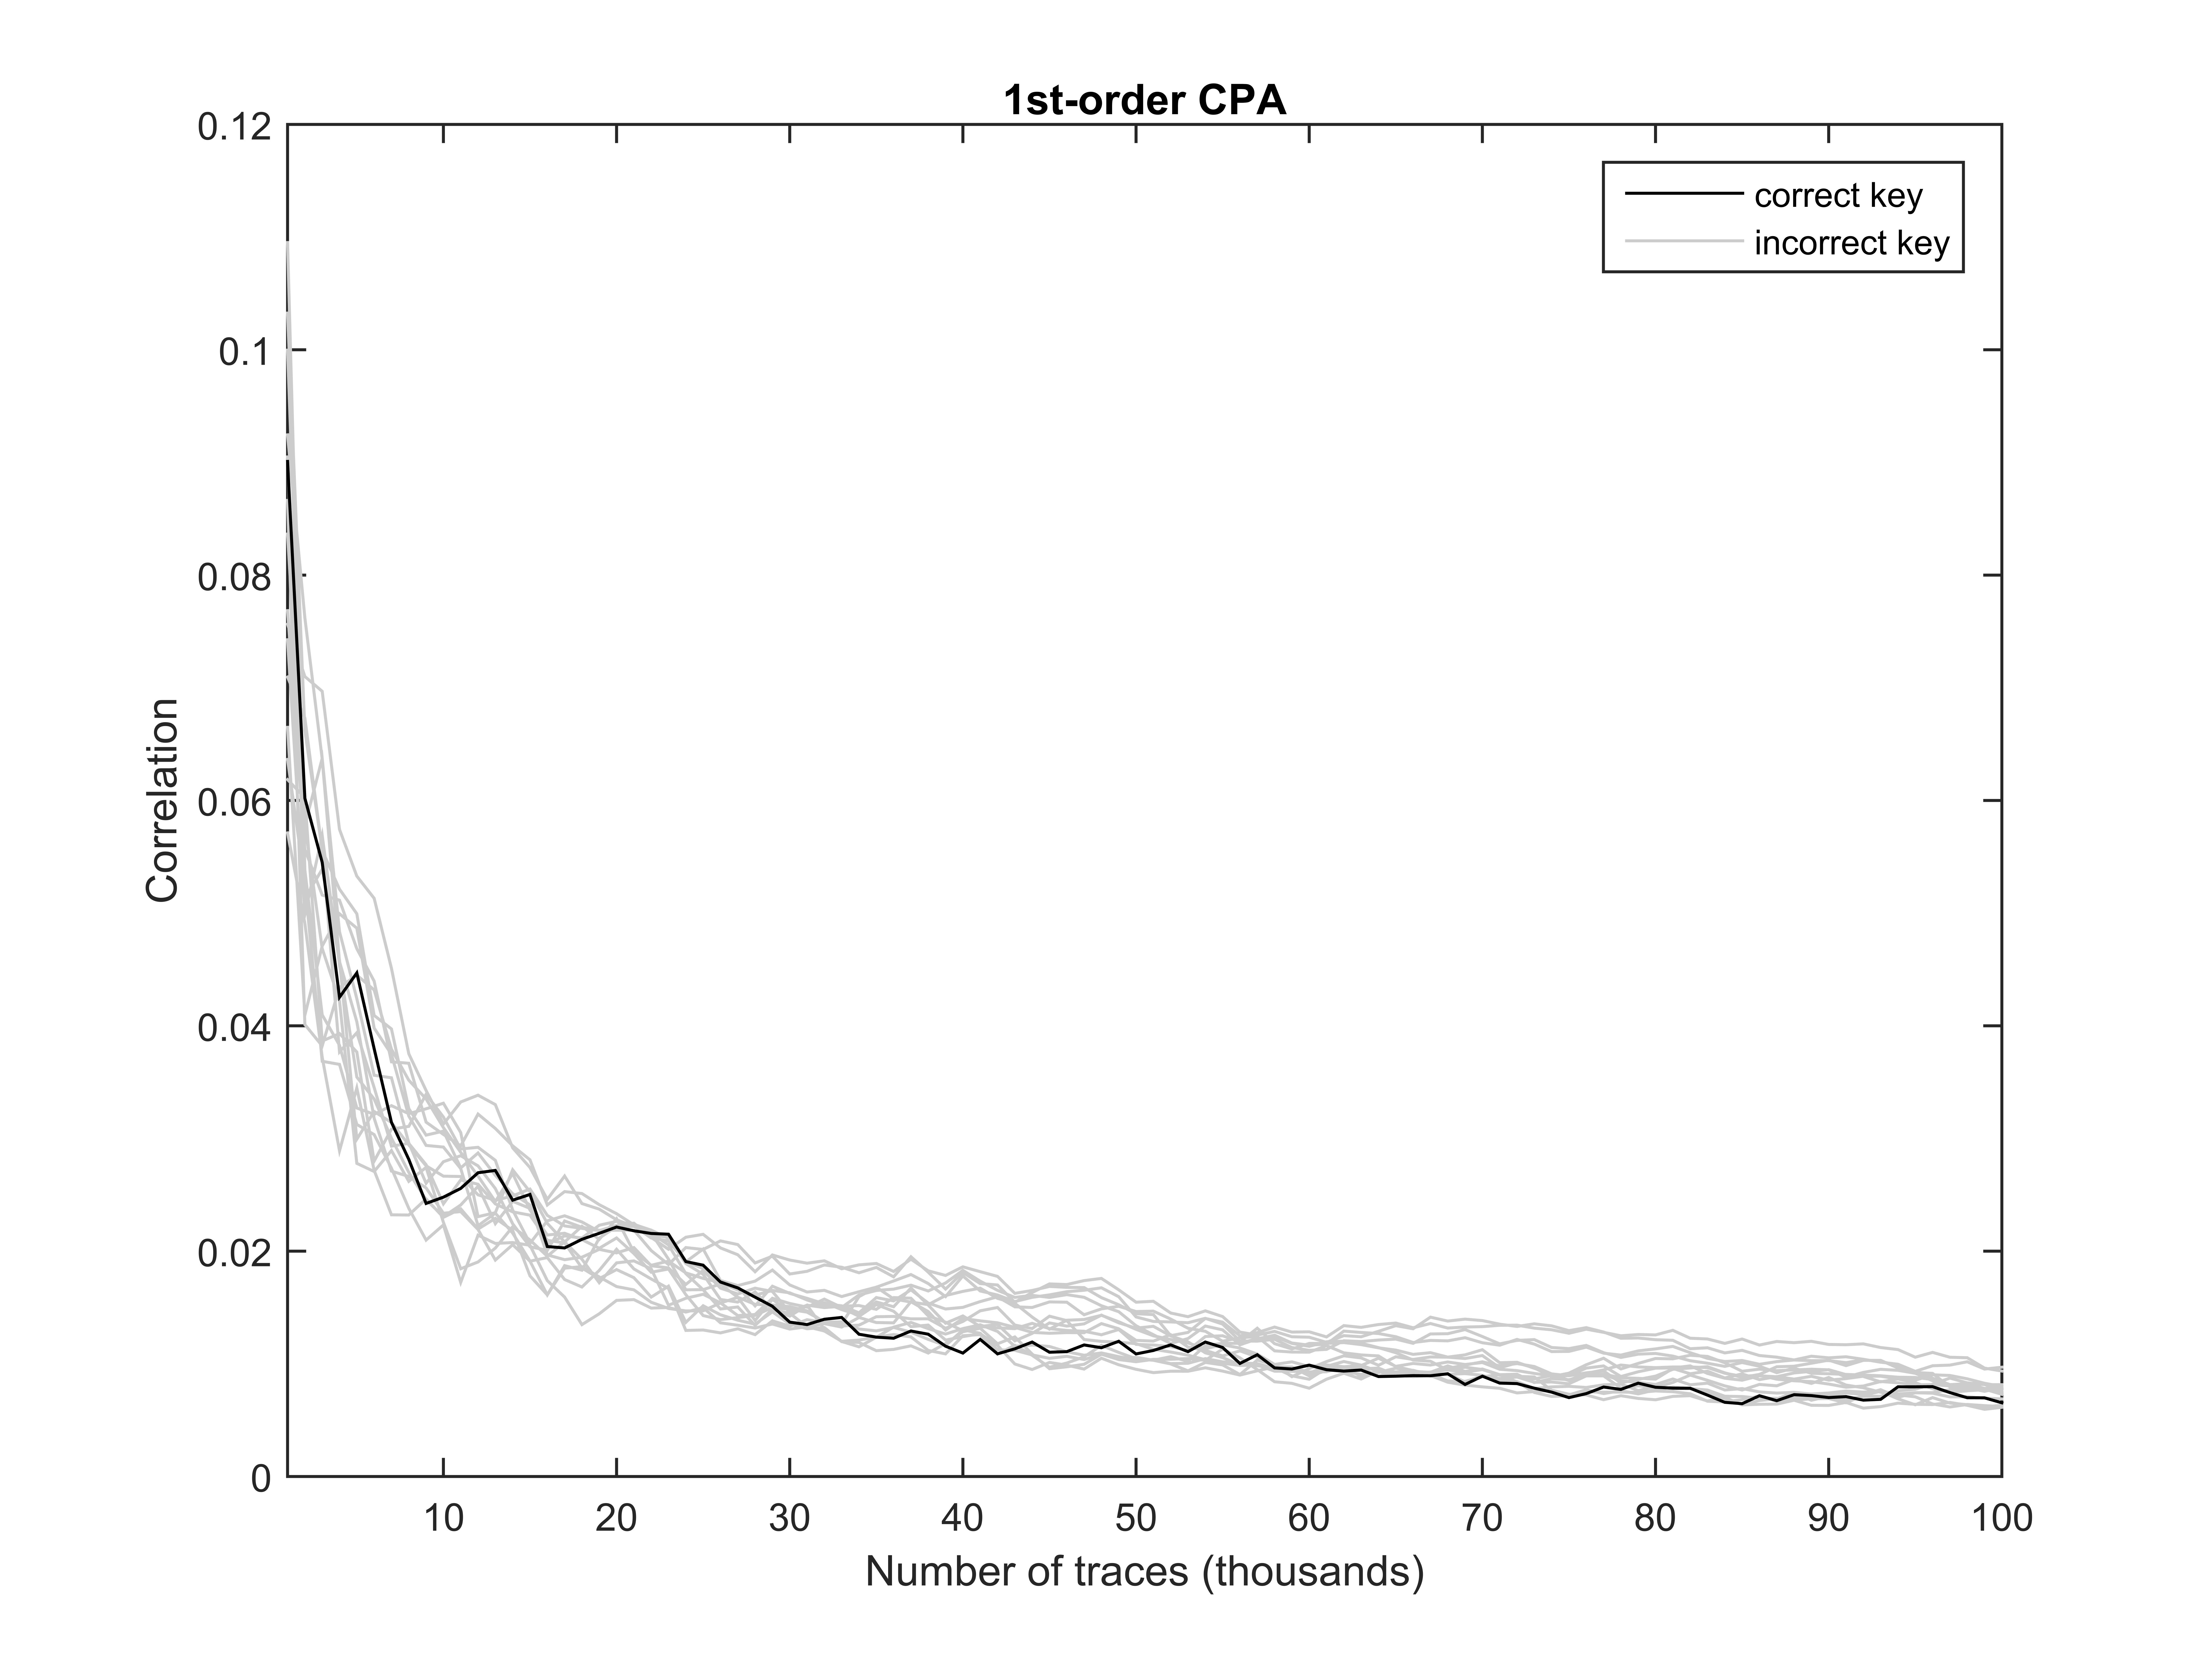
\includegraphics[width=\textwidth]{{fig/clear_rem_cpa.png}}

        \caption{\scriptsize{Clearing remnant effect,1st-order CPA, HW model, 100k traces.}}
\label{fig:clear_rem_cpa}
    \end{subfigure}  \hspace{15px}
 \begin{subfigure}[b]{0.40\textwidth}
       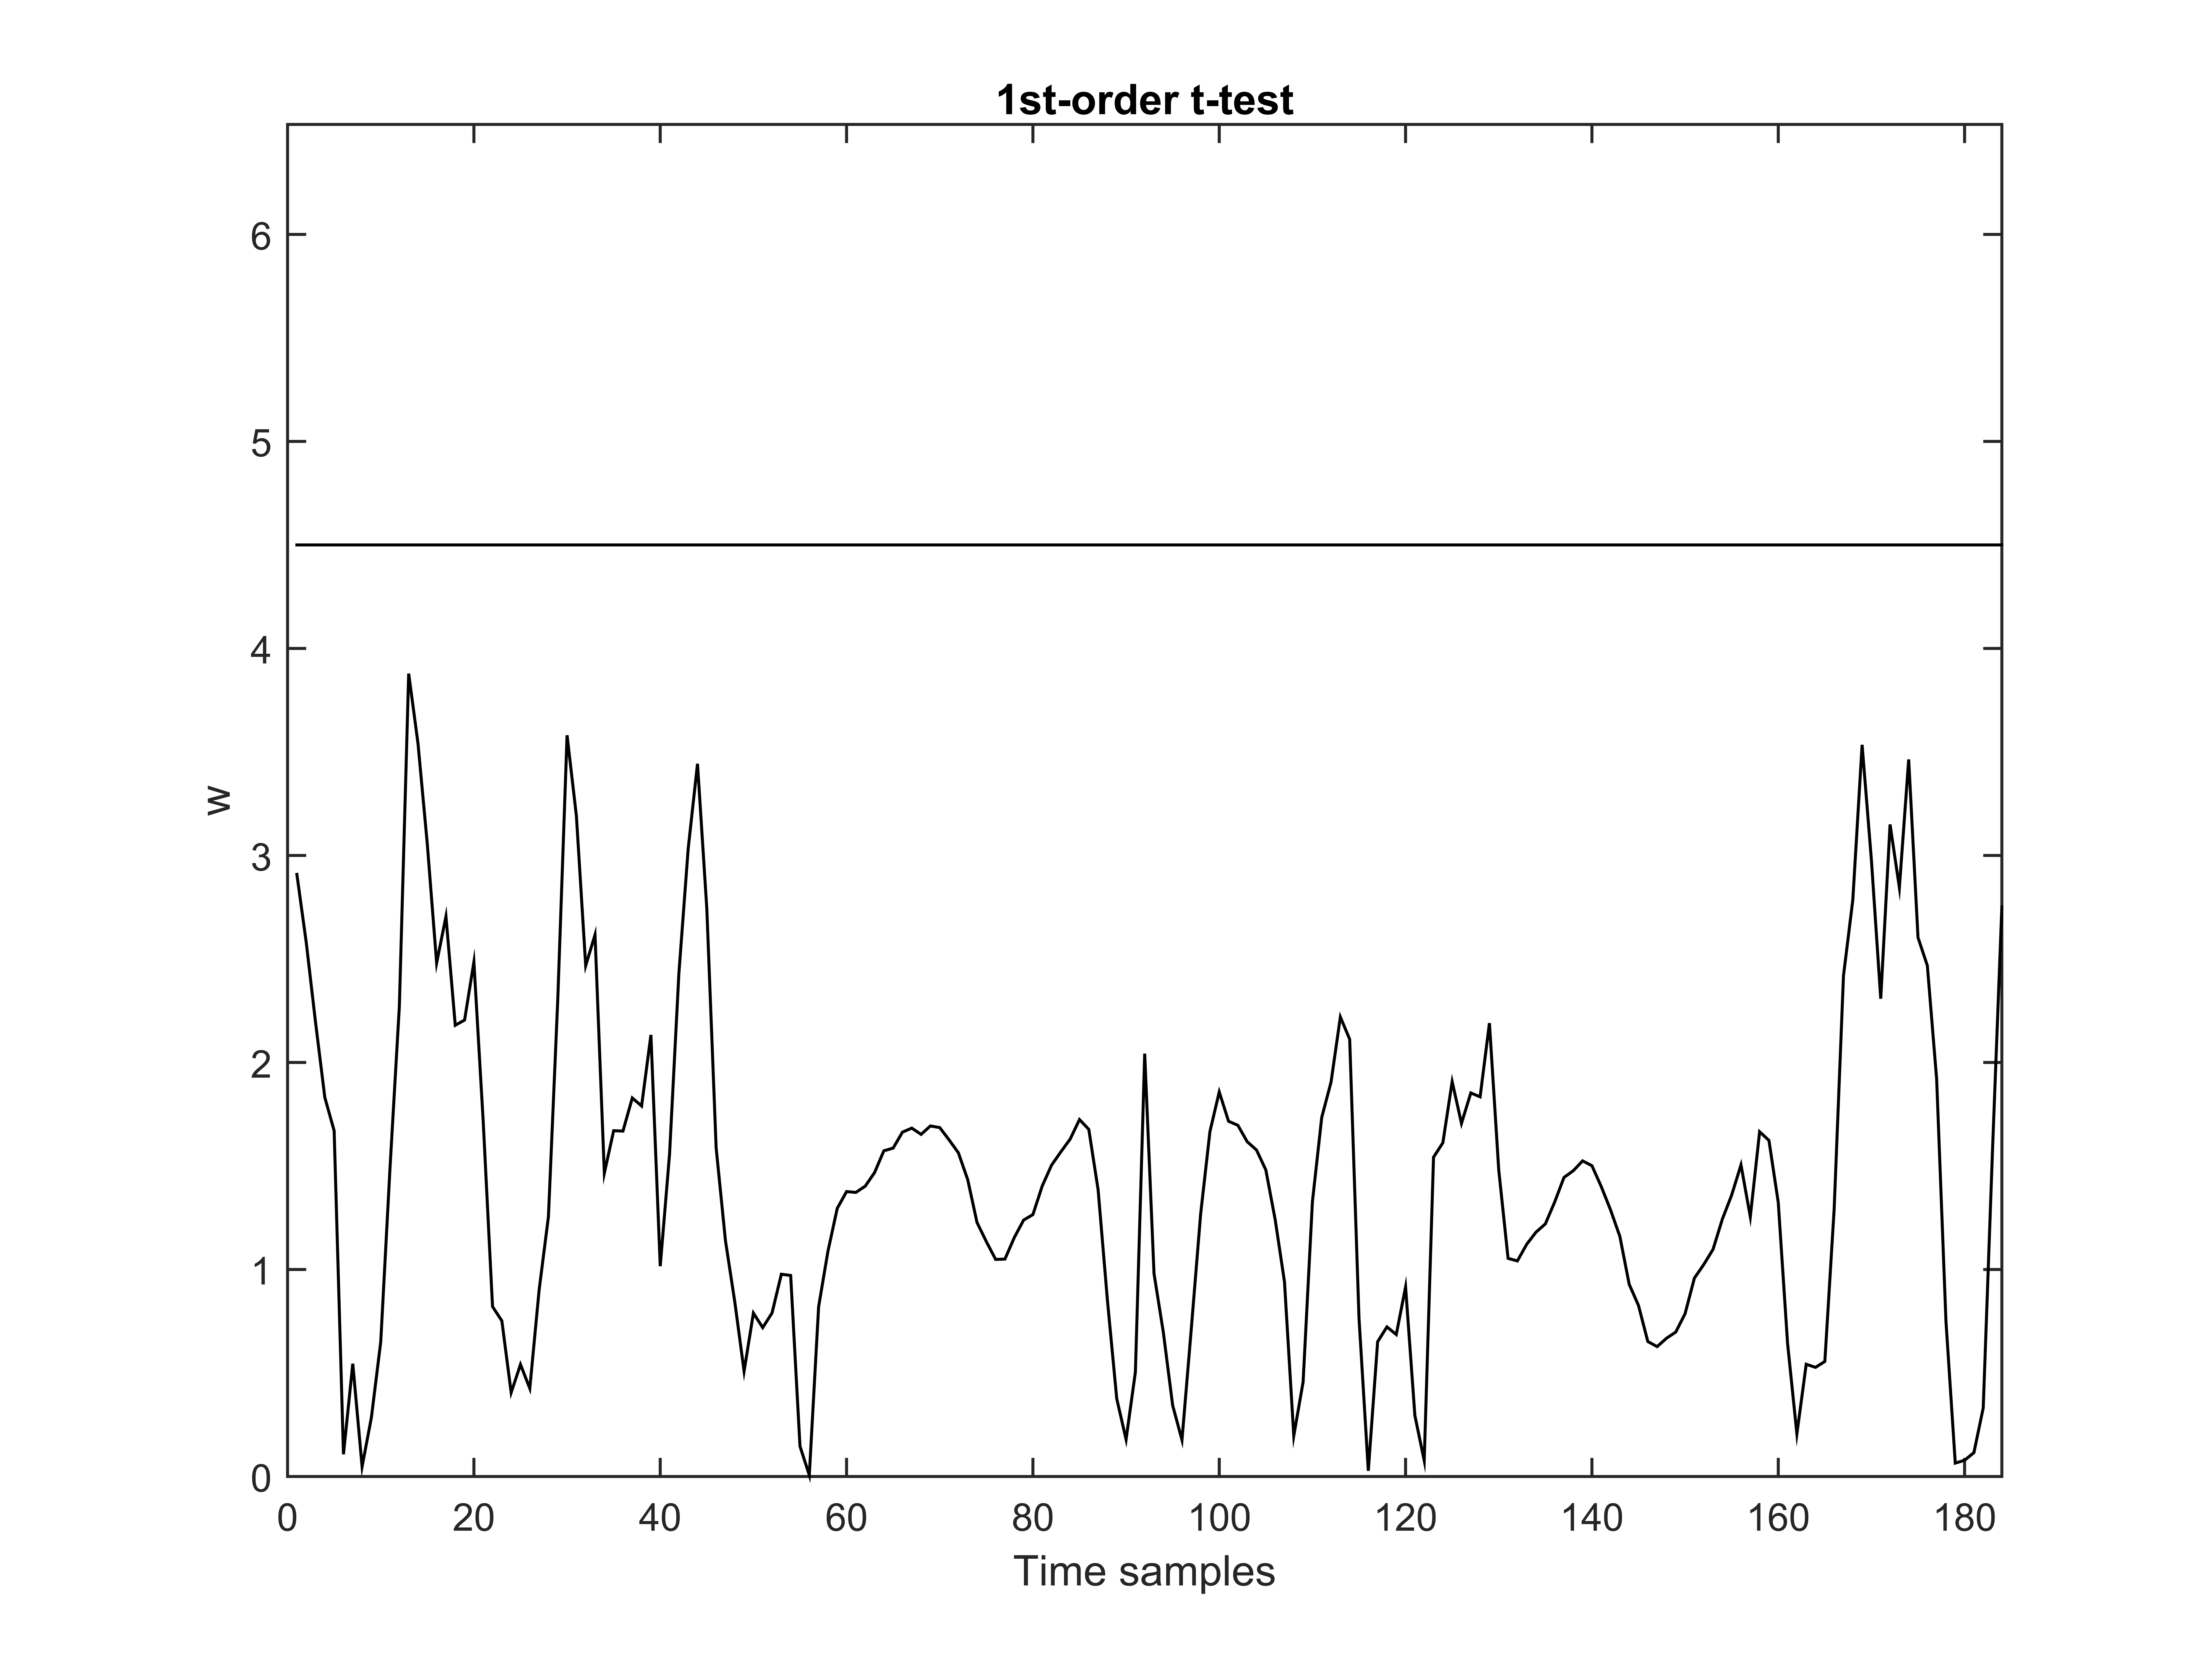
\includegraphics[width=\textwidth]{{fig/clear_rem_t.png}}

        \caption{\scriptsize{Clearing remnant effect, 1st-order t-test, 100k random vs. 100k fixed.}}
\label{fig:clear_rem_t}
    \end{subfigure}

   
    \caption{Memory-based remnant effect}\label{fig:regleak}
\end{figure}
\end{subsection}
We address the remnant scenario with two experiments. Listing \ref{lst:remnant} demonstrates how two consecutive SRAM accesses \texttt{ld rA, SRAM\_x0}, followed by \texttt{ld rB, SRAM\_x1} produce the remnant effect. Second, in Listing \ref{lst:clearing_remnant}, we show how clearing the register and accessing an unrelated SRAM address (\texttt{0x0085}) can remove the remnant. 

As shown in Figures \ref{fig:mem_rem_cpa}, \ref{fig:mem_rem_t}, consecutive SRAM accesses can potentially lead to ILA violations. Exploiting (in a univariate manner) the memory remnant effect in ATMega163 needs less than 500 traces with our setup. Preventing the effect requires the clearing of the register and the insertion of a dummy SRAM access. Alternatively, the implementor could ensure that same-family shares are not accessed sequentially. Note also that the \texttt{st} instruction produces a similar effect.
\begin{subsection}{Neighbour Leakage Effect}\label{combined_leakage}
The neighbour leakage effect implies that accessing or processing the contents of a data storage unit will cause leakage in another unit as well. For example, assume that share $x_0$ is stored in register \texttt{rB} and share $x_1$ is being processed in register \texttt{rA}. Assume also that the registers \texttt{rA, rB} are subject to the neighbour leakage effect. Processing \texttt{rB} will produce a value-based leakage of $x_0$. At the same time, the neighbouring leakage effect will cause \texttt{rA} to leak the value of $x_1$, resulting in the combined leakage of both shares and the recovery of sensitive value $x$. The following two experiments (Listing \ref{lst:combined_leakage}) verify the neighbour leakage effect between registers \texttt{r2, r3}, i.e. that a share stored in \texttt{r2} leaks when manipulating \texttt{r3} and vice-versa. 

%\begin{figure}[H]
%    \centering
%\begin{subfigure}[b]{0.4\textwidth}
%\texttt{;clear all registers\\
%;store x0 in r2 \\
%mov r0, r0\\
%NOPs \\
%mov r1, r1\\
%NOPs \\
%mov r2, r2\\
%NOPs \\
%mov r3, r3 \\
%NOPs \\
%...\\
%mov r31, r31 }

%        \caption{\scriptsize{Neighbour leakage \texttt{r2-r3}.}}
%\label{fig:r23_exp}
%    \end{subfigure}
%\begin{subfigure}[b]{0.4\textwidth}
%\texttt{;clear all registers\\
%;store x0 in r3 \\
%mov r0, r0\\
%NOPs \\
%mov r1, r1\\
%NOPs \\
%mov r2, r2\\
%NOPs \\
%mov r3, r3 \\
%NOPs \\
%...\\
%mov r31, r31 }

%        \caption{\scriptsize{Neighbour leakage \texttt{r3-r2}.}}
%\label{fig:r32_exp}
%    \end{subfigure}
%\caption{Neighbour leakage experiments}
%\end{figure}
\lstset{caption={Neighbour leakage experiment for \texttt{r2} and \texttt{r3}.},label=lst:combined_leakage}
\begin{lstlisting}
; clear all registers
; x is in the selected register (r2 OR r3)
mov r0, r0
nop ; x5
mov r1, r1
nop ; x5 
mov r2, r2 @\label{line:r2}@
nop ; x5
mov r3, r3 @\label{line:r3}@
nop ; x5
...
mov r31, r31 
\end{lstlisting}
\begin{figure}

 \begin{subfigure}[b]{0.40\textwidth}
        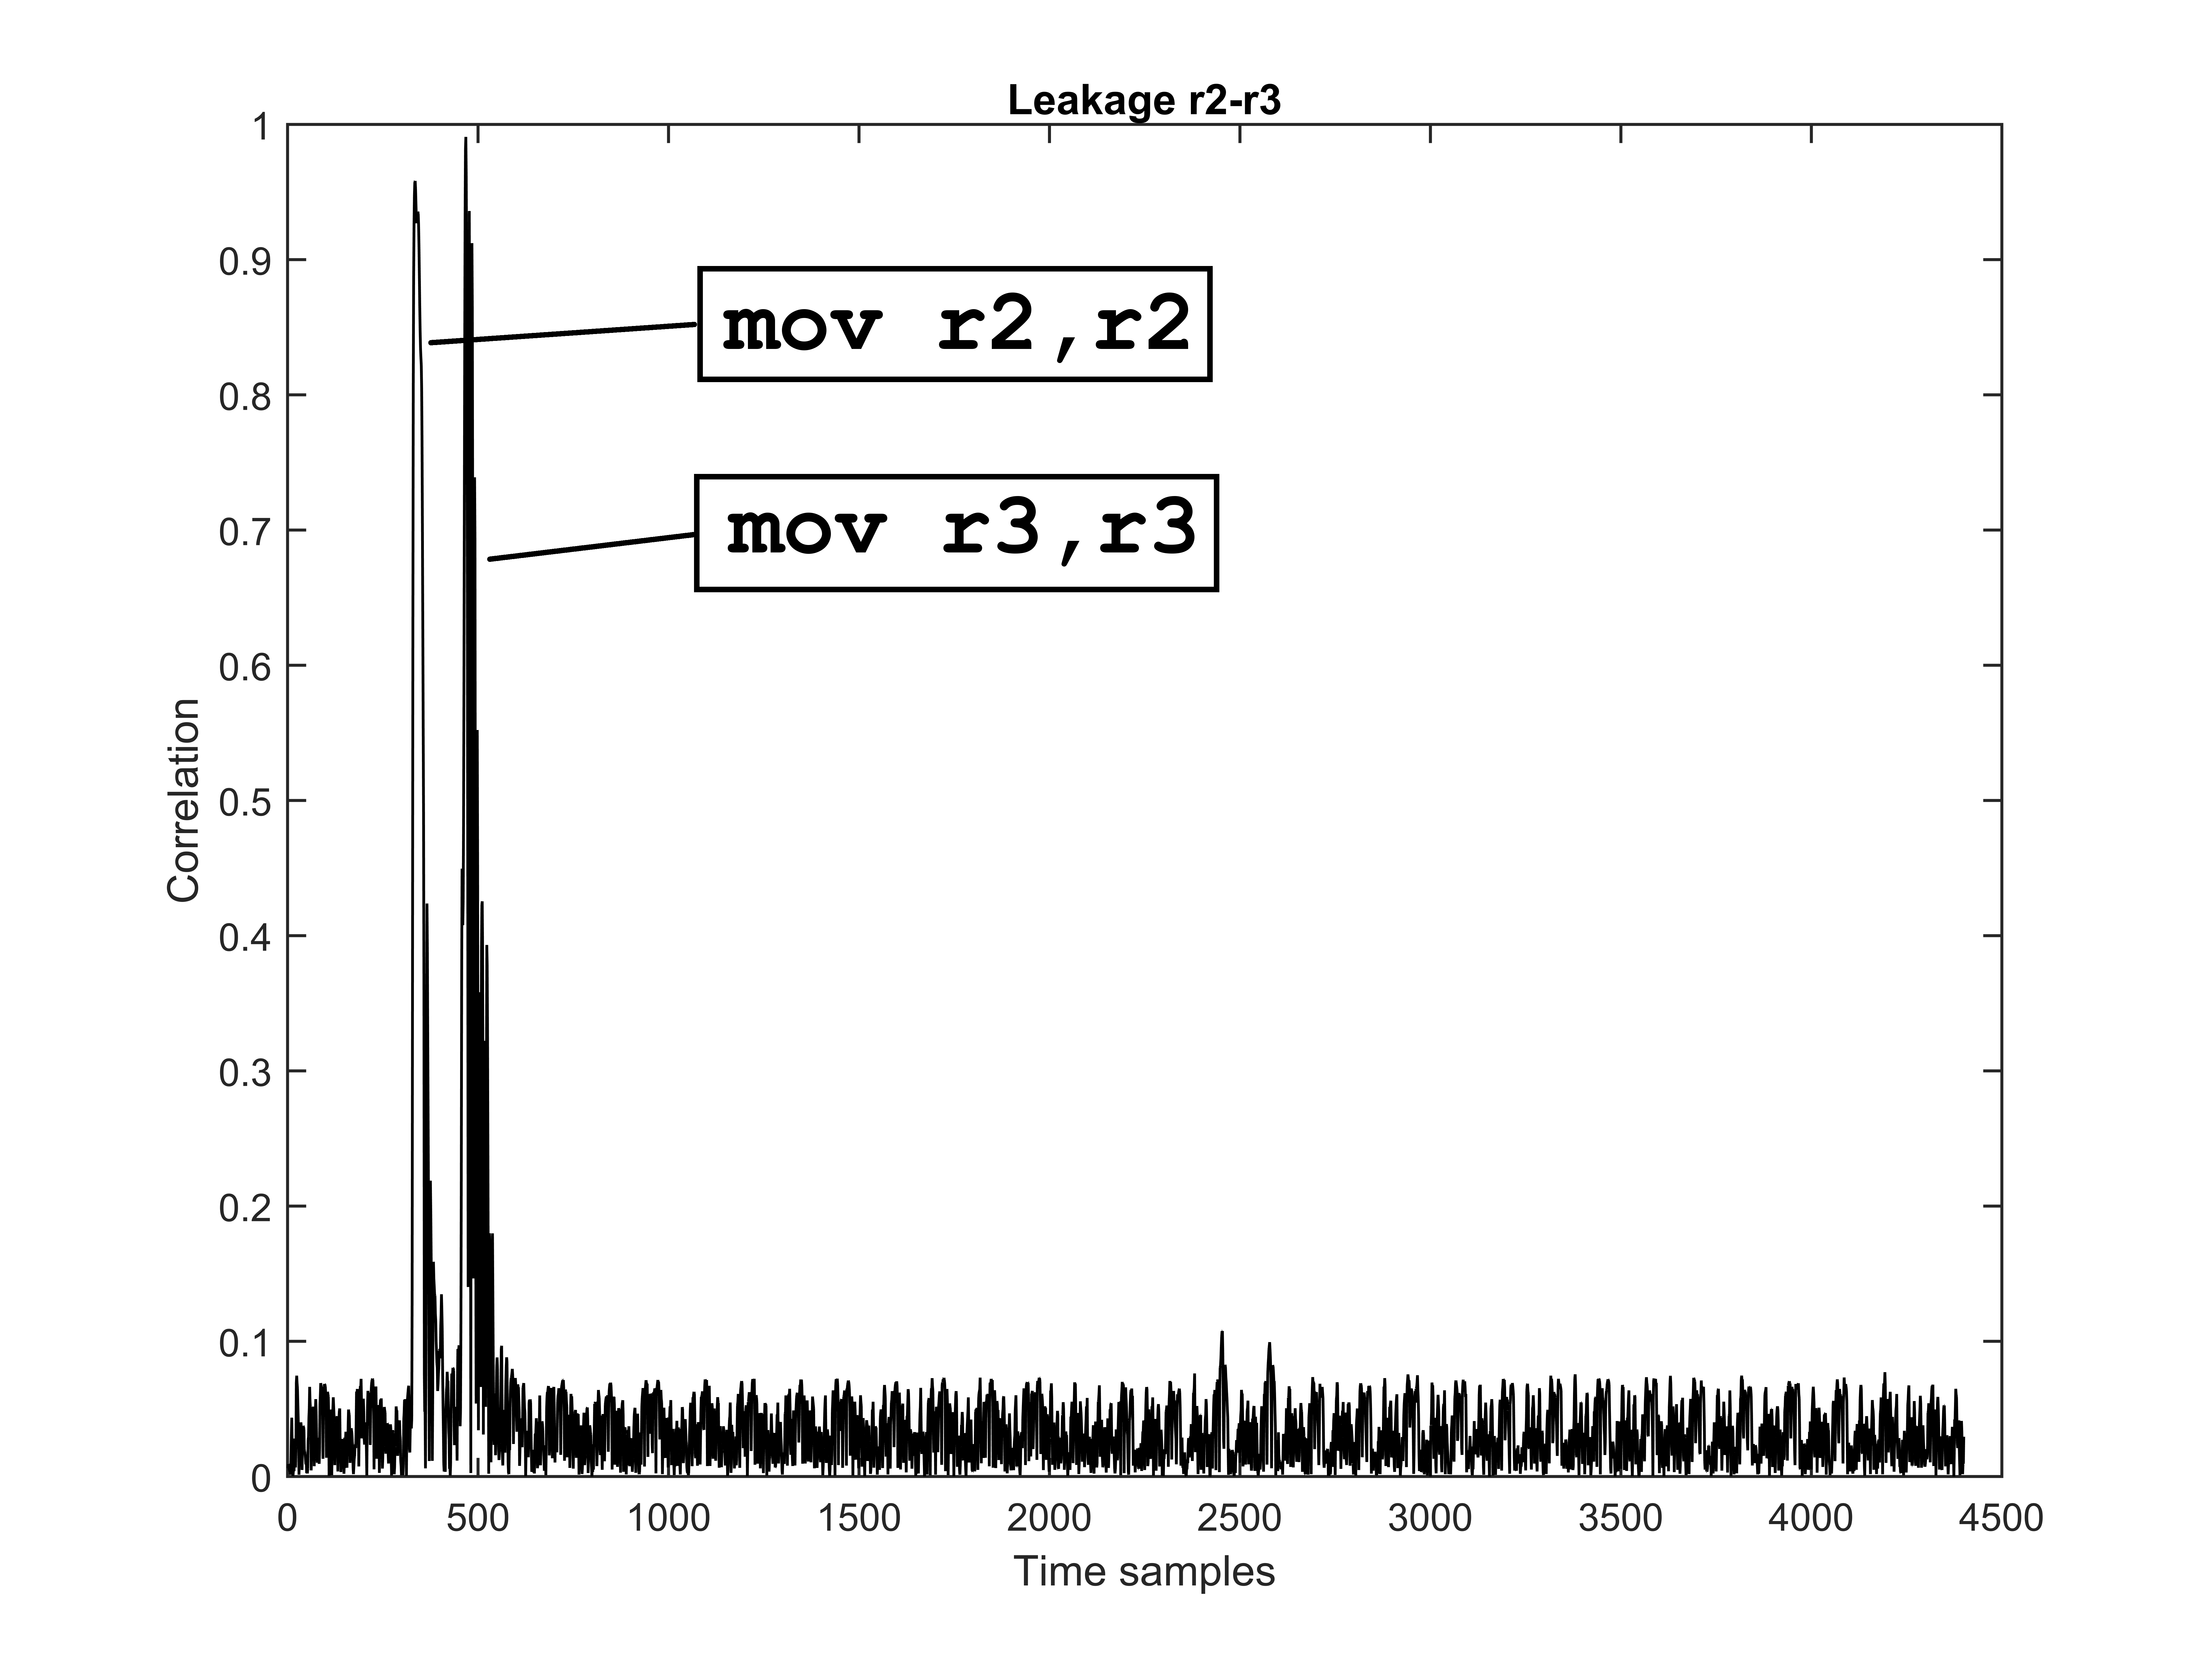
\includegraphics[width=\textwidth]{{fig/corr_r23_an.png}}

        \caption{\scriptsize{Correlation $\rho(HW(x_0),traceset)$, \texttt{r2-r3}, 5k traces.}}
\label{fig:corr23}
    \end{subfigure} \hspace{15px}
 \begin{subfigure}[b]{0.40\textwidth}
        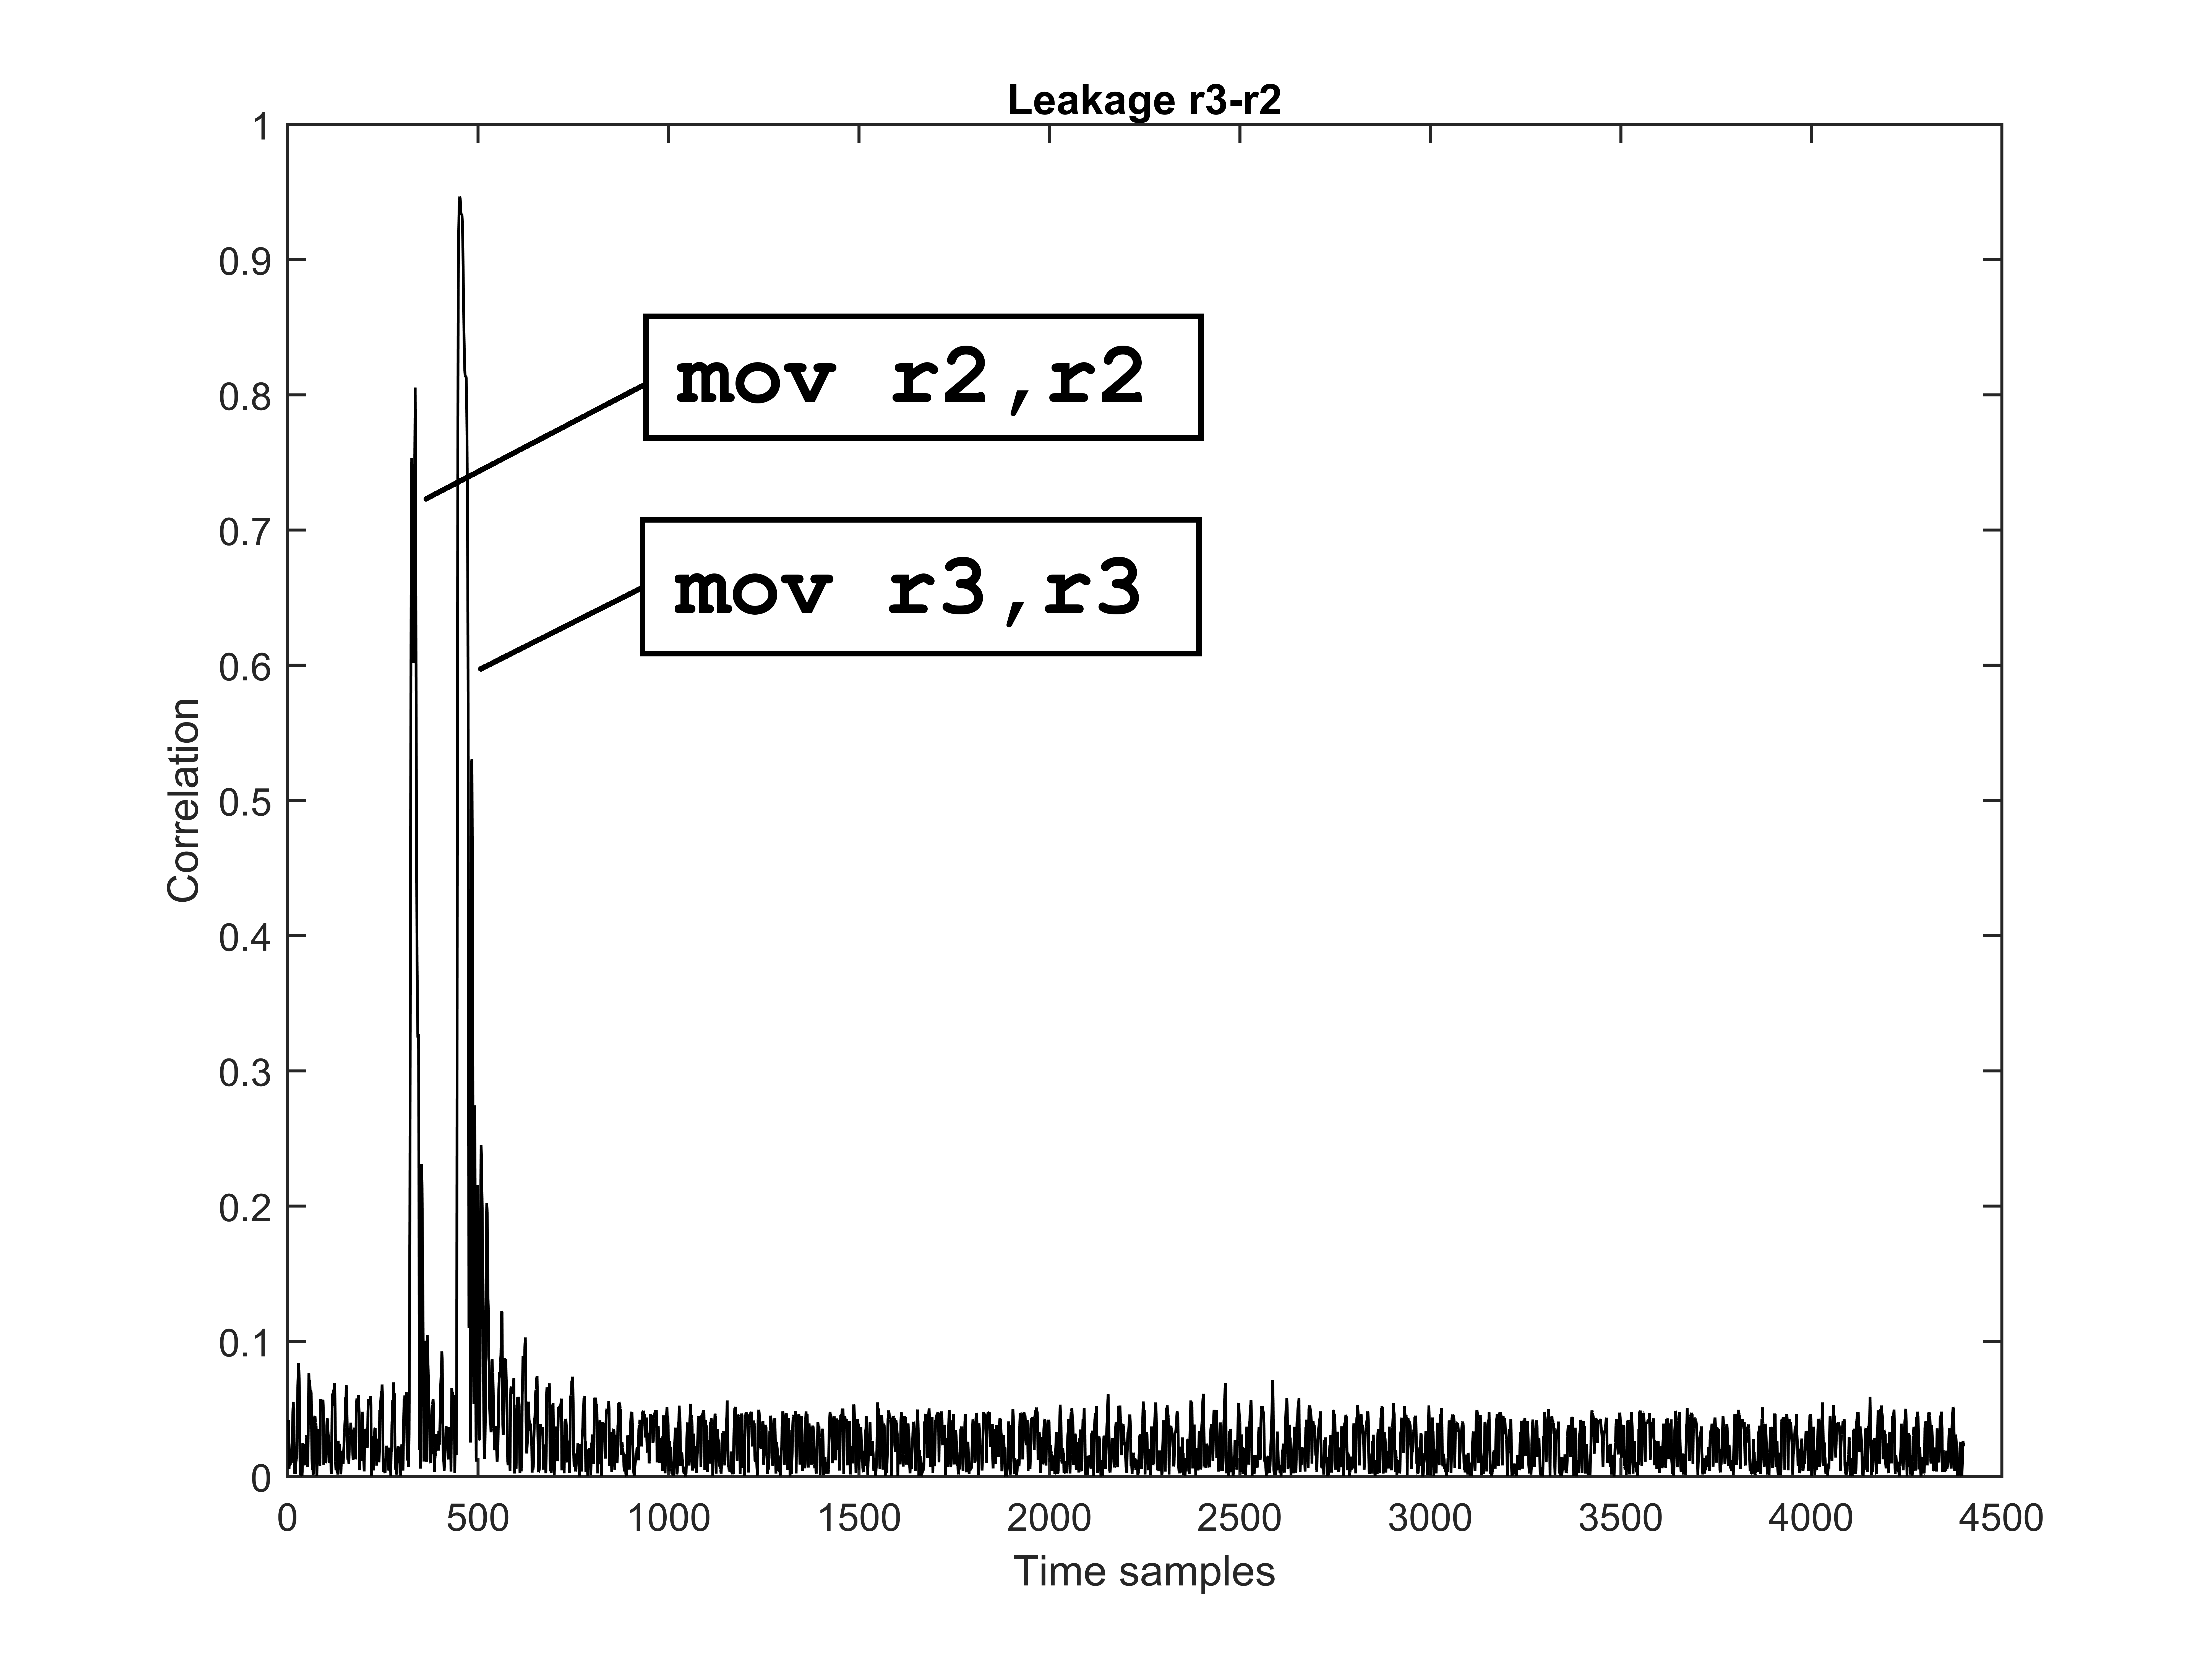
\includegraphics[width=\textwidth]{{fig/corr_r32_an.png}}

        \caption{\scriptsize{Correlation $\rho(HW(x_0),traceset)$, \texttt{r3-r2}, 5k traces.}}
\label{fig:corr32}
    \end{subfigure}

   
    \caption{Neighbour-based leakage effect}\label{fig:regleak}
\end{figure}

As shown above, we use the same code from Listing \ref{combined_leakage}, but in the first time we put the sensitive variable $x$ into register \texttt{r2} (\emph{only} line~\ref{line:r2} should result in leakage).
In the second time, we put the sensitive value into the register \texttt{r3} (\emph{only} line~\ref{line:r3} should leak).
As a result, we have identified a pair of data storage units (\texttt{r2,r3}) that exhibit the neighbour leakage effect. Note that in this case the effect is symmetrical, i.e. \texttt{r2} triggers \texttt{r3} and vice-versa (Figures \ref{fig:corr23},\ref{fig:corr32}). We also observed that the effect is persistent, i.e. the \texttt{mov} instructions will trigger the same behavior, even if performed later. We run the same experiment in order to identify all possible neighbour leakages in the register file (all pairs in set $\{$\texttt{r0,...,r31}$\}$). The results are available in the Appendix, matrix $R$. The issue mostly affects consecutive registers, although exceptions exist, e.g. register \texttt{r0}. We did not identify a similar effect in SRAM memory, yet our experiments were limited to a small region of cells. As a solution to the neighbour effect, the developer can opt to avoid storing shares in such registers. Alternatively, he can store all shares in SRAM, except for the ones currently in use. 
\end{subsection}\\\\\\
Summing up, we stress the following focal points regarding the ILA-breaching effects and their solutions:
\begin{itemize}
\item All identified effects are device-dependent, i.e. there is no hard guarantee that they are observable and reproducible in different AVR-based microcontrollers, let alone different architectures such as ARM, TI, PIC etc. Both intra-AVR and inter-architectural observability of the effects remains open.
\item The effects are often counter-intuitive when viewed in the assembly layer of abstraction. They originate from the hardware and/or the physical layer, thus can only be detected via experimental evaluation. Linking the assembly ILA-breaching effects to a particular hardware component or physical phenomenon is non-trivial~\cite{DBLP:conf/eurocrypt/RenauldSVKF11,DBLP:phd/dnb/Stottinger12}, especially without knowledge of the underlying chip architecture and properties.
\item  Since the effect's detection requires experimental evaluation, different instructions or code arrangements can potentially lead to additional, unidentified ILA-breaching effects. Still, we maintain that it is possible to construct ``hardened" masked operations in ATMega163 by removing the identified effects (see Section \ref{sec:rectangle}). It remains open whether the suggested solutions are computationally optimal or more efficient clearing techniques can be identified.
\end{itemize}

The takeaway message of this section is that assembly-level soundness cannot enforce ILA and hence 1st-order security, due to the nature of the breaching effects. However, it is possible to acquire sufficient knowledge about effects and solutions in a particular device. These non-intuitive checks discussed above can be subsequently integrated into a code-checking tool which can identify such effects in assembly code.

\section{Detection Tool}\label{sec:tool}

Several tools that can help designers of cryptographic systems
were already suggested and discussed in literature.

SILK~\cite{DBLP:conf/acsac/Veshchikov14} presented in 2014
can be used to generate simulated traces based on C++ code, it allows
to generate sets of traces on early stages of development in order to test an implementation
against any attack. However, SILK works only with C++ high level source code and 
can not take into account reordering of instructions that is often used by compilers during
optimisation. Also, this tool does not detect flaws in implementations, 
it only allows to easily generate simulated traces that can be used for tests.

A tool based on formal verification 
was presented at EUROCRYPT in 2015~\cite{DBLP:conf/eurocrypt/BartheBDFGS15},
it can detect design flaws in masking schemes.
This tool can analyse programs written using EasyCrypt framework and its language,
it requires a designer to transform the original implementation (e.g., in assembly or C code)
to EasyCrypt. Unfortunately, errors cound potentially be introduced during this process
and there is no garantee that the programm written using EasyCrypt will be equivalent
to the programm in the original programming language, the the best of our knowledge
free automated tools that can transform C or assembly programms to EasyCrypt do not exist.
Moreover, this tool is not opensource and thus can not be used by any developer.

A simulation tool based tool that can be used to analyse masking implementations
was presented at FSE in 2016~\cite{DBLP:conf/fse/Reparaz16}.
It can be used with software and hardware implementations
and it requires only the high-level implementation source code such as C.
Due to this fact it can be blind to rearangements of opperations 
(which can lead to side-channel leakage) created by the compiler.
Up until now, the source code of this tool also remaines unavailable for general public.


\todo[inline]{Our tool}



\section{Hardened 1st-order Masked Sbox for RECTANGLE}\label{sec:rectangle}
We have discussed the ILA-breaching effects in Section \ref{sec:ila_effects} and integrated these observations in the ASCOLD tool,  described in Section \ref{sec:tool}. The current Section builds up on these advances by putting forward a ``hardened", 1st-order masked, ISW-based RECTANGLE Sbox. The desired aim is to produce an assembly-based, lightweight Sbox implementation that is secure against 1st-order, univariate attacks, hence forcing the attacker to resort to 2nd-order and/or multivariate techniques. 

Our implementation opts for a bitsliced~\cite{DBLP:conf/fse/DaemenGV93,DBLP:conf/fse/Biham97a} representation, due to both the bitsliced structure of RECTANGLE and to the $GF(2)$-oriented nature of the ISW countermeasure. We employ a bitslicing factor of 2, i.e. we exploit the 8-bit AVR architecture in order to process two 4-bit Sboxes in parallel (nibble-slicing). The Sbox is decomposed into $GF(2)$ operations which can be accelerated by via SIMD-like, 8-bit assembly instructions. The decomposition suggested by Zhang et al.~\cite{DBLP:journals/chinaf/ZhangBLR0V15} is optimal w.r.t. $GF(2)$ multiplicative complexity, since Grosso et al.~\cite{DBLP:conf/fse/GrossoLSV14} established that the minimum number of non-linear operations required by 4x4 Sboxes is 4. 

In order to ``harden" the Sbox, we use the solutions suggested in Section \ref{sec:ila_effects} and follow two approaches: efficient and conservative. In the \emph{efficient} approach, after processing any share, we clear the registers on a need-to basis and insert dummy \texttt{ld} instructions to avoid overwrite and remnant effects. We avoid neighbouring leakage effects by always storing the shares in SRAM, i.e. the register file contains only the shares used by the current instruction. In the \emph{conservative} approach, we perform all the afore-mentioned clearing techniques. In addition, we insert dummy \texttt{st} instructions and perform thorough register/memory clearing. Both efficient and conservative approaches are applied to every single instruction of the implementation, i.e. the cost is linear w.r.t. the number of instructions that manipulate masked shares. The resulting computational overhead is significant: the efficient ``hardened" Sbox implementation runs in 993 clock cycles, i.e. almost 12 times slower compared to the ``naive" 1st-order, ISW-based RECTANGLE Sbox, which runs in $87$ clock cycles. The conservative ``hardened" Sbox implementation requires 1319 clock cycles, i.e. it is 15 times slower. Table \ref{cc_table} contains a comparison between ``naive" 1st-order, ``naive" 2nd-order and efficient/conservative ``hardened" 1st-order bitsliced implementations of the RECTANGLE Sbox in AVR assembly.
\begin{table}[H]
\centering
\caption{Masked Sbox comparison in ATMega163}
\label{cc_table}
\begin{tabular}{ |l|l|l|l|l|}
\hline
\textbf{Order $\mathbf{d}$} & \textbf{Hardened} & \textbf{Latency (cc) }& \pbox{20cm}{ \textbf{Throughput} \\ \textbf{(bits/cc $\mathbf{*10^{-3}}$)} }& \textbf{RNG (bytes)} \\ \hline \hline 
Unprotected  & no & 32 & 250 & 0 \\ \hline
1st order      &   no & 87 & 91 &  4\\ \hline
 1st order      &   yes (eff.)& 993 & 8 & 4\\ \hline
 1st order      &   yes (cons.) & 1319 & 6 & 4\\ \hline
 2nd order     &   no  & 775 & 10 & 12\\ \hline
\end{tabular}
\end{table}

Using the 1st-order, random vs. fixed t-test, we evaluate the efficient and conservative ``hardened" 1st-order Sboxes, as well as the ``naive" 1st-order Sbox. Using a $25$k random vs. $25$k fixed t-test does not yield any statistically significant leakage in the efficient ``hardened" version (Figure \ref{hardbox_eff}). However, wenote that a $50$k random vs. $50$k fixed t-test is able to detect leakage, i.e. trying to reduce the cost of enforcing ILA can have a detrimental effect on security. For the conservative ``hardened" Sbox, a 100k random vs. 100k fixed t-test does not detect any leakage (Figure \ref{hardbox_cons}). Note that a \emph{2nd-order} $25$k random vs. $25$k fixed t-test on a chosen sample window is able to detect leakage. Therefore, we conclude that for the given device, the informativeness of 1st-order attacks is substantially limited and a 2nd-order attack is the preferable adversarial strategy (Figure \ref{t_order2}). Naturally, the ``naive" 1st-order version rejects the null hypothesis (Figure \ref{softbox}) due to the ILA-breaching effects and the 1st-order leakage can be easily exploited.
\begin{figure}[H]

 \begin{subfigure}[b]{0.40\textwidth}
        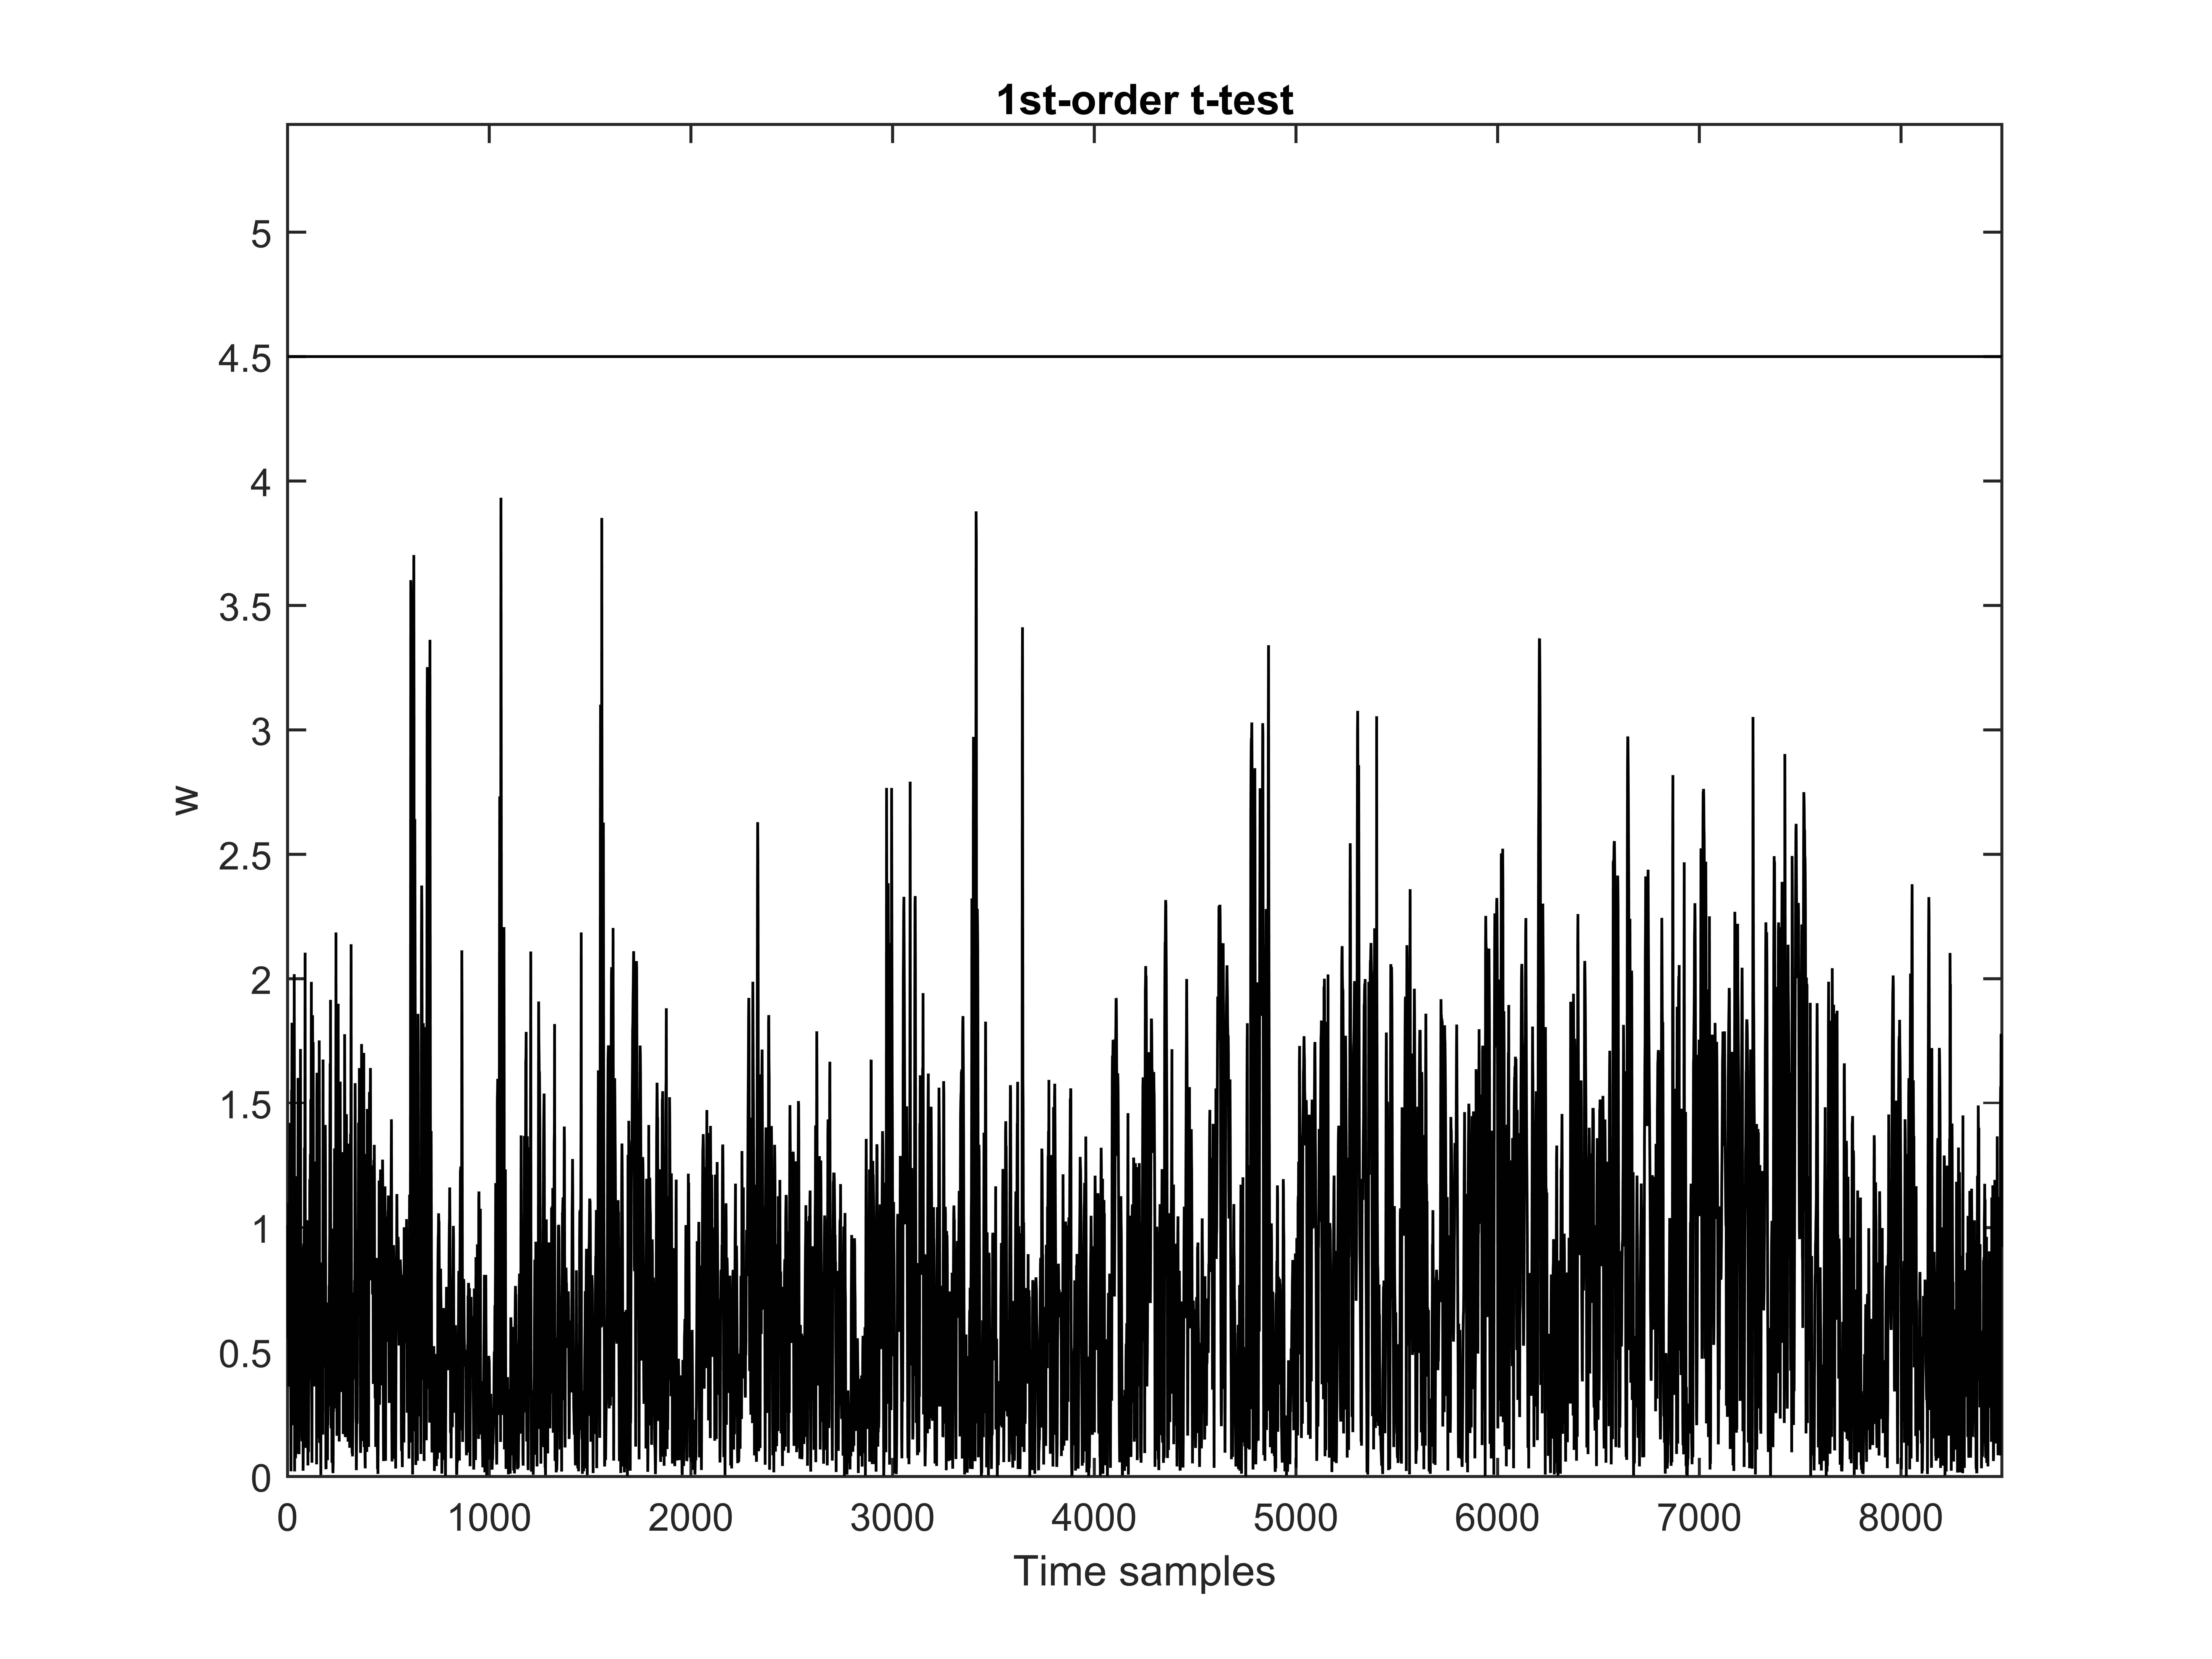
\includegraphics[width=\textwidth]{{fig/hardbox_eff.png}}

        \caption{\scriptsize{Efficient hardened Sbox, 1st-order t-test, 25k random vs. 25k fixed.}}
\label{hardbox_eff}
    \end{subfigure}  \hspace{15px}
 \begin{subfigure}[b]{0.40\textwidth}
        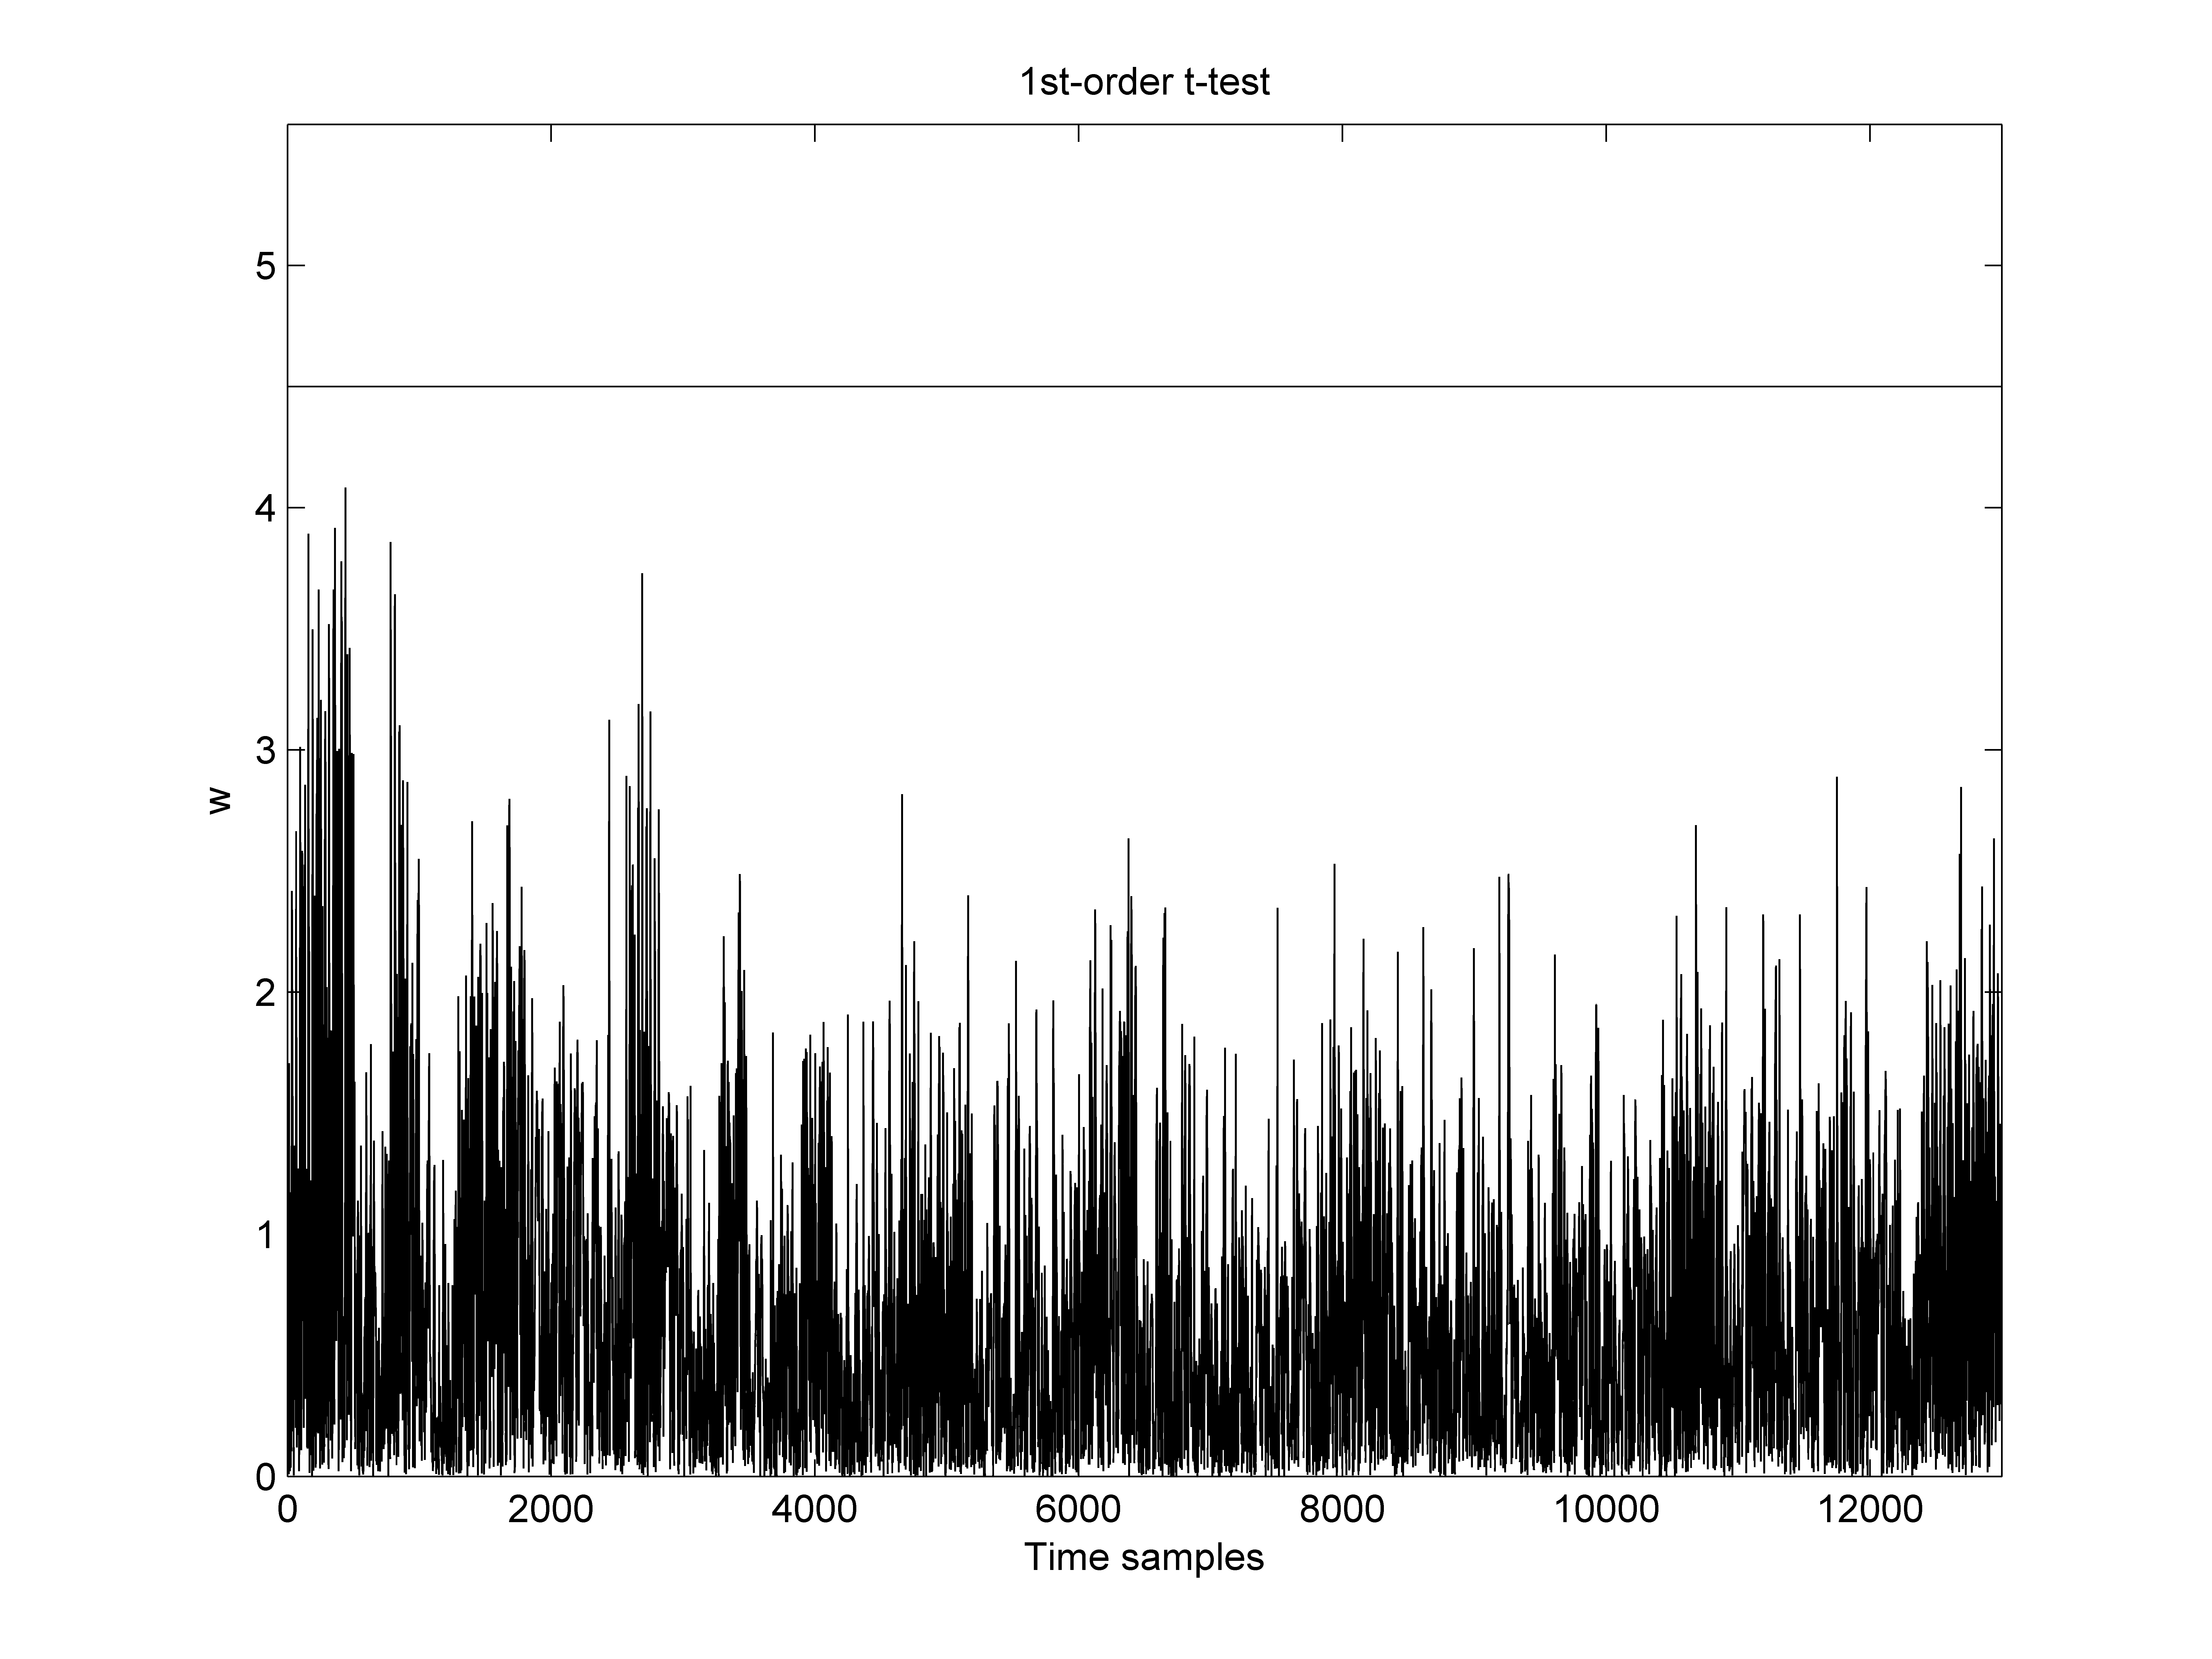
\includegraphics[width=\textwidth]{{fig/hardbox_cons.png}}

        \caption{\scriptsize{Conservative hardened Sbox, 1st-order t-test, 100k random vs. 100k fixed.}}
\label{hardbox_cons}
    \end{subfigure}

\begin{subfigure}[b]{0.40\textwidth}
        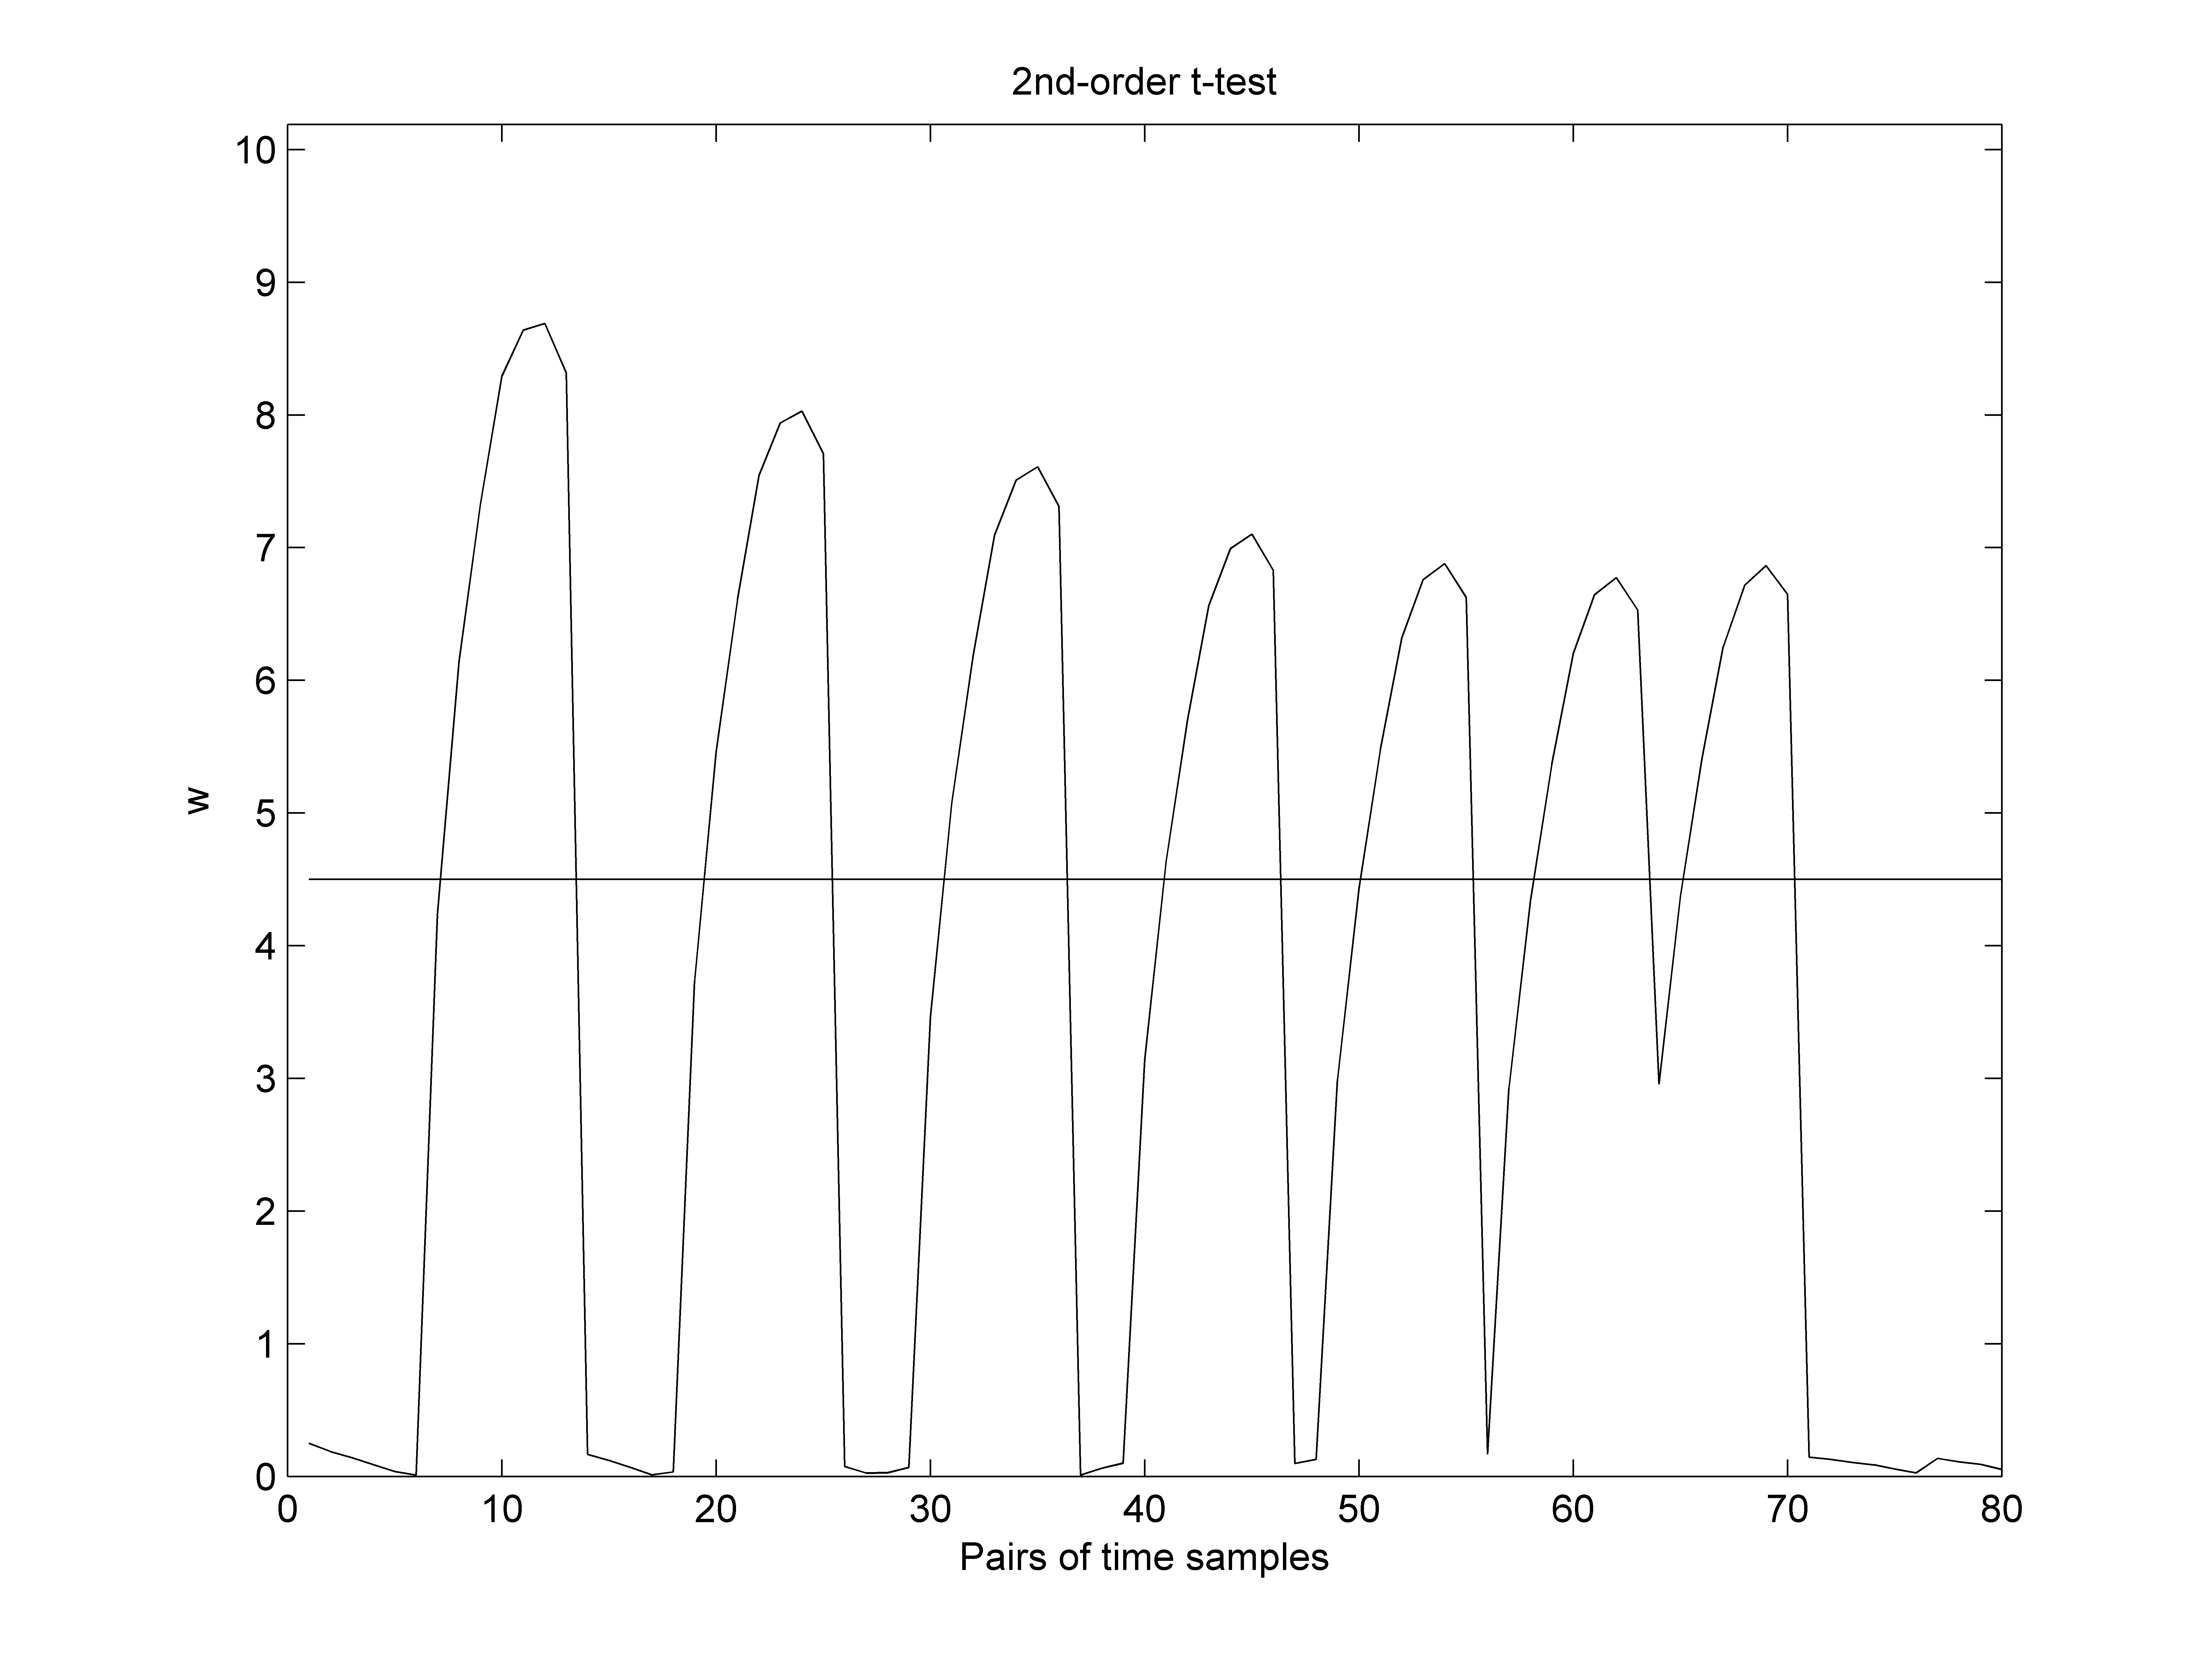
\includegraphics[width=\textwidth]{{fig/t_order2.png}}

        \caption{\scriptsize{Consevative hardened Sbox, 2nd-order t-test, 25k random vs. 25k fixed.}}
\label{t_order2}
    \end{subfigure} \hspace{15px}
 \begin{subfigure}[b]{0.40\textwidth}
        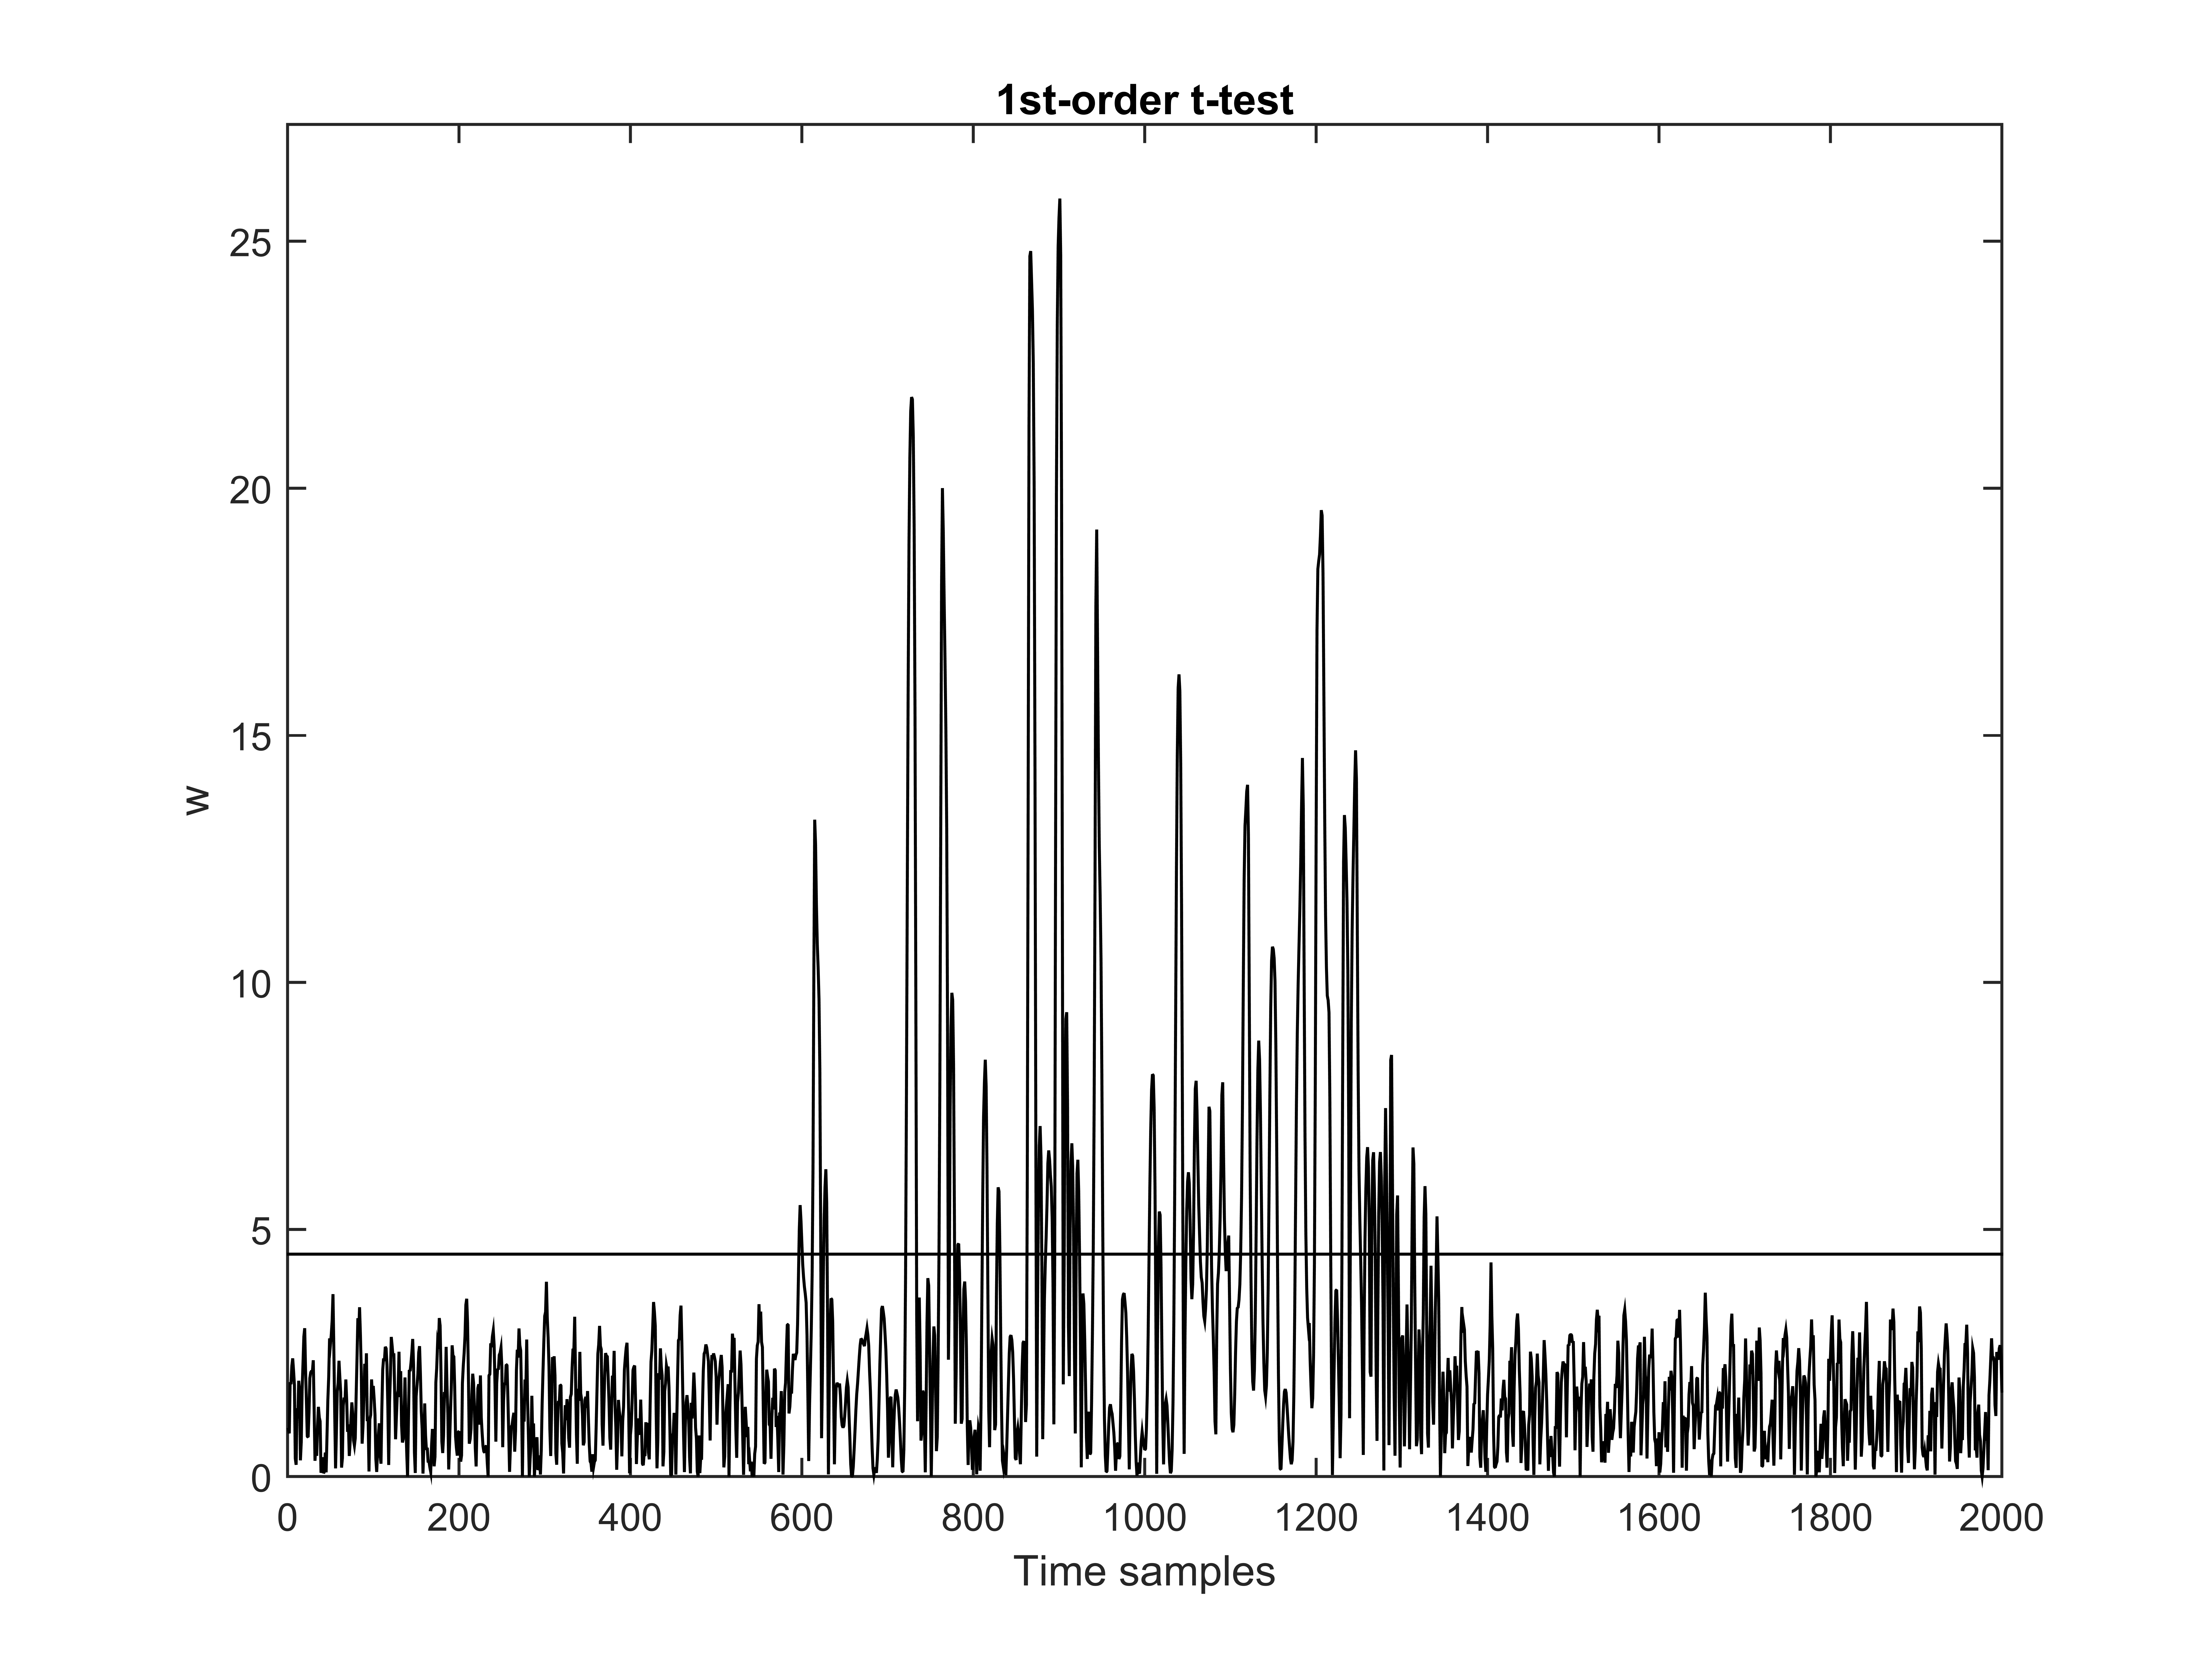
\includegraphics[width=\textwidth]{{fig/softbox.png}}

        \caption{\scriptsize{Naive Sbox, 1st-order t-test, 1k random vs. 1k fixed.}}
\label{softbox}
    \end{subfigure}

   
    \caption{Hardened and naive Sbox evaluations}\label{fig:sboxleak}
\end{figure}
So far, the only way to guarantee the actual security order of a real-world implementation was to increase the scheme's theoretical order $d$, in order to ensure that the implementation attains an actual order of $\lfloor \frac{d}{2} \rfloor$~\cite{DBLP:conf/cardis/BalaschGGRS14, DBLP:journals/iacr/GrootPPSB16}. Clearing the ILA-breaching effects requires a significant overhead and is device-dependent, yet it is the only technique known to us that can enforce 1st-order, univariate security. In addition, hardening does not increase the scheme order $d$, thus the random number generation (RNG) cost is not increased. The previous suggestions require a higher scheme order, hence a significant overhead, since both the implementation cost and the RNG cost are quadratic w.r.t. the order. We compare the ``hardened" 1st-order and ``naive" 2nd-order implementation costs (in clock cycles) and we observe that hardening the 1st-order Sbox is slower than increasing the scheme's order from 1 to 2 (both in the efficient and in the conservative case). Still, the solution requires no extra RNG and we maintain that removing these effects can also be beneficial to higher-order implementations, i.e. it is complimentary to masking. The extent to which higher-order implementations can benefit from removing such effects remains an open problem.



















\section{Conclusions} \label{sec:conclusions}

This work investigated the hazards in software masking, suggested a verification tool and established a secure, 1st-order masked Sbox implementation against 1st-order, univariate attacks. Still, several important questions for future work arise. We demonstrated that removing the ILA-breaching effects is feasible, yet identifying the best clearing mechanism and minimizing the overhead is a topic for further exploration. Similarly, the current work is limited in AVR ATMega163 and needs to be extended to different devices and platforms. Moreover, higher-order evaluation techniques are still nascent and in this work we did not focus on 1st-order, yet multivariate attacks such as those that exploit horizontality~\cite{DBLP:conf/ches/BattistelloCPZ16}. In addition, note that the ILA effects are observable throughout an implementation. Not only the cipher-related operations but any manipulation of shares during I/O, RNG routines etc. can create hazards. Thus, there is need for effort towards a fully hardened implementation. Last but not least, we stress that the effects identified depend on the architecture and the physical layer, thus preventing them in the assembly layer is, in principle, less efficient and prone to errors. Ideally, we should strive towards custom-made microcontrollers that enforce ILA in hardware, without the addition of countermeasures such as threshold implementations~\cite{DBLP:conf/icics/NikovaRR06}.  

%\section{Acknowledgments}
%Do we have any?

\bibliography{research}

\end{document}
% end of file template.tex

